\documentclass{beamer}
% \mode<presentation>
\setbeamertemplate{navigation symbols}{}
\let\tempone\itemize
\let\temptwo\enditemize
\renewenvironment{itemize}{\tempone\addtolength{\itemsep}{0.5\baselineskip}}{\temptwo}
\usepackage{beamerthemeshadow}
\usepackage{ulem}
\usepackage{tikz}
\usepackage{hyperref}
\usepackage{natbib}
\usepackage{pgffor}
\usepackage{booktabs}
\usepackage{graphicx}
\usepackage{amssymb}
\usepackage{tabularx}
\usepackage{tikz,etoolbox}
\usepackage{tikz,amsmath,siunitx}
\usetikzlibrary{arrows,snakes,backgrounds,patterns,matrix,shapes,fit,calc,shadows,plotmarks}

\usepackage{subcaption}
% \usepackage{url}
% \usepackage{hyperref}
\usepackage{pgf}
\usepackage{latexsym}
\usepackage{amsfonts}
\usepackage{amssymb}
\usepackage{amsthm}
\usepackage{algorithm}
\usepackage{amsmath}
\usepackage{tabularx}
\usepackage{xcolor}
\usepackage[absolute,overlay]{textpos}
\usetikzlibrary{shapes,arrows,positioning,automata,positioning,spy,matrix,scopes,chains}
\newcommand{\digs}[2]{\hphantom{999}\llap{#1}\,+\,\hphantom{999}\llap{#2}}
\setbeamersize{text margin left=6mm}
\setbeamersize{text margin right=6mm}
\renewcommand{\insertnavigation}[1]{}
\setbeamertemplate{headline}{}
\setbeamertemplate{footline}{}
\usefonttheme{professionalfonts}
% make itemize things larger
%\setbeamerfont*{itemize/enumerate body}{size=\Large}
%\setbeamerfont*{itemize/enumerate subbody}{size=\large}
\setbeamercovered{transparent}
\mode<presentation>
%\mode<handout>
\linespread{1.25}
\DeclareMathOperator{\Tr}{Tr} 

\usepackage{color}
\usepackage{multirow}
\usepackage{rotating}
\usepackage[all,dvips]{xy}
\usepackage{colortbl}
\usepackage{graphicx}
\usepackage{verbatim}
\usepackage{framed}
\usepackage{natbib}
\usepackage[labelformat=empty]{caption}
\newcommand{\air}{\vspace{0.25cm}}
\newcommand{\mair}{\vspace{-0.25cm}}

\setbeamertemplate{navigation symbols}{}%remove navigation symbols
\renewcommand{\rmdefault}{crm}
\newcommand{\lnbrack}{{\normalfont [}}
\newcommand{\rnbrack}{{\normalfont ]}\thinspace}
\newcommand{\lbbrack}{\textcolor{red}{\textbf{[}}}
\newcommand{\rbbrack}{\textcolor{red}{\textbf{]}}\thinspace}
\definecolor{vermillion}{RGB}{213,94,0}
\newcommand{\given}{\,|\,}
\definecolor{orange}{RGB}{230,159,0}
\definecolor{skyblue}{RGB}{86,180,233}
\definecolor{bluegreen}{RGB}{90,143,41}
% \definecolor{bluegreen}{RGB}{0,158,115}
\definecolor{myyellow}{RGB}{240,228,66} % i dunno if this is the same as standard yellow
\definecolor{myblue}{RGB}{0,114,178}
\definecolor{vermillion}{RGB}{213,94,0}
\definecolor{redpurple}{RGB}{204,121,167}
\definecolor{lightgrey}{RGB}{234,234,234}

\newcommand{\ha}{\boldh_{\ua}}
\newcommand{\hp}{\boldh_{\up}}
\newcommand{\hc}{\boldh_{\mathrm{c}}}



\usetikzlibrary{positioning}
% \setbeamerfont{alerted text}{series=\bfseries}
% \setbeamerfont{structure}{series=\bfseries}
% Needed for diakgrams.
\def\im#1#2{
  \node(#1) [scale=#2]{\pgfbox[center,top]{\pgfuseimage{#1}}
};}
% \input{pictures_header}


\title[Seq2seq]{Interpreting, Training, and Distilling Seq2Seq Models}


\author[Alexander Rush]{Alexander Rush  (@harvardnlp) \\  
{\scriptsize  (with  Yoon Kim, Sam Wiseman, Allen Schmaltz, Sebastian Gehrmann, Hendrik Strobelt) } \\} 

\institute[Harvard SEAS]{ \\
  \begin{center}
    
\includegraphics[width=1.7cm]{seas}
  \end{center}
  at \\ 
  \begin{center}
    
\includegraphics[width=2cm]{twitter}
  \end{center}
  
}
\date{}
% \usetheme{Madrid}

\newcommand{\enc}{\mathrm{src}}
\newcommand{\xvec}{\mathbf{x}}
\newcommand{\yvec}{\mathbf{y}}
\newcommand{\wvec}{\mathbf{w}}
\newcommand{\cvec}{\mathbf{c}}
\newcommand{\zvec}{\mathbf{z}}
% \newcommand{\mcY}{\mathcal{Y}}
% \newcommand{\mcV}{\mathcal{V}}
\newcommand{\context}{\mathbf{w}_{\mathrm{c}}}
\newcommand{\embcontext}{\mathbf{\tilde{w}}_{\mathrm{c}}}
\newcommand{\inpcontext}{\mathbf{\tilde{x}}}
\newcommand{\start}{\mathbf{\tilde{y}}_{\mathrm{c0}}}
\newcommand{\End}{\mathrm{\texttt{</s>}}}

\newcommand{\Uvec}{\mathbf{U}}
\newcommand{\Evec}{\mathbf{E}}
\newcommand{\Gvec}{\mathbf{G}}
\newcommand{\Fvec}{\mathbf{F}}
\newcommand{\Pvec}{\mathbf{P}}
\newcommand{\pvec}{\mathbf{p}}
\newcommand{\Qvec}{\mathbf{Q}}
\newcommand{\Vvec}{\mathbf{V}}
\newcommand{\Wvec}{\mathbf{W}}
\newcommand{\hvec}{\mathbf{h}}
% \newcommand{\reals}{\mathbb{R}}

\newcommand{\Cite}[1]{{\footnotesize \citep{#1}}}
\newcommand{\TT}[1]{{\footnotesize\tt{#1}}}
\newcommand{\boldw}{\boldsymbol{w}}
\newcommand{\boldu}{\boldsymbol{u}}
\newcommand{\boldv}{\boldsymbol{v}}
\newcommand{\boldb}{\boldsymbol{b}}
\newcommand{\boldW}{\boldsymbol{W}}
\newcommand{\boldh}{\boldsymbol{h}}
\newcommand{\boldg}{\boldsymbol{g}}
\newcommand{\ua}{\ensuremath{\mathrm{a}}}
\newcommand{\up}{\ensuremath{\mathrm{p}}}
%\newcommand{\bphi}{\ensuremath{\mathbf{\phi}}}
\newcommand{\bphi}{\boldsymbol{\phi}}
\newcommand{\btheta}{\boldsymbol{\theta}}
\newcommand{\mcY}{\mathcal{Y}}
\newcommand{\mcX}{\mathcal{X}}
\newcommand{\mcC}{\mathcal{C}}
\newcommand{\mcA}{\mathcal{A}}
\newcommand{\mcV}{\mathcal{V}}
\newcommand{\trans}{\ensuremath{\mathsf{T}}}
\def\argmin{\operatornamewithlimits{arg\,min}}
\def\argmax{\operatornamewithlimits{arg\,max}}
\newcommand{\reals}{\ensuremath{\mathbb{R}}}

\newcommand{\aphi}{\boldsymbol{\phi}_{\mathrm{a}}}
\newcommand{\pwphi}{\boldsymbol{\phi}_{\mathrm{p}}}
\newcommand{\squigaphi}{\widetilde{\boldsymbol{\phi}}_{\mathrm{a}}}
\newcommand{\squigpwphi}{\widetilde{\boldsymbol{\phi}}_{\mathrm{p}}}

\newcommand{\aW}{\boldW_{\mathrm{\ua}}}
\newcommand{\pW}{\boldW_{\mathrm{\up}}}

\newcommand{\ab}{\boldb_{\mathrm{\ua}}}
\newcommand{\pb}{\boldb_{\mathrm{\up}}}

\newcommand{\Da}{d_{\mathrm{a}}}
\newcommand{\Dp}{d_{\mathrm{p}}}

% \newcommand{\ha}{\boldh_{\ua}}
% \newcommand{\hp}{\boldh_{\up}}

\newcommand{\ourmodel}{This work}
\newcommand{\zro}{{\color{white}0}}


\def\argmax{\operatornamewithlimits{arg\,max}}
\def\kargmax{\operatornamewithlimits{K-arg\,max}}

\begin{document}

\begin{frame}
  \titlepage
\end{frame}
  \note{
    Thank you for inviting me today. It is an honor to 
    give a talk here at the Center for Language And Speech Technology.}


% % \begin{frame}{Introduction}
% %   \begin{columns}
% %     \begin{column}{0.7\textwidth}
      
% %       \structure{Previous:}
% %       \begin{itemize}
% %       \item \structure{Degree:} 
% %         \begin{itemize}
% %         \item MIT with Prof. Michael Collins
% %         \item Visiting Scholar at Columbia University
% %         \end{itemize}
% %       \item \structure{Intern:}
% %       \begin{itemize}
% %       \item Google NLP Research (NYC)
% %       \end{itemize}
% %     \item\structure{Post-Doc}
% %       \begin{itemize}
% %       \item Facebook AI Research Lab (NYC) 
% %       \item Group run by Yann LeCun
% %       \end{itemize}

% %       \end{itemize}
% %       \structure{Assistant Professor} at Harvard SEAS
% %       \begin{itemize}
% %       \item CS182: Artificial Intelligence
% %       \item CS287: Natural Language Processing
% %       \end{itemize}


% %     \end{column}
% %     \begin{column}{0.3\textwidth}
% %       \begin{center}    
% %         \includegraphics[width=3cm]{pic1}
% %       \end{center}
% %     \end{column}
% %   \end{columns}
% % \end{frame}


% % \begin{frame}{Contents}
% %   \tableofcontents
% % \end{frame}

% \section{Deep Learning For Language}


% \begin{frame}% {Deep Learning in NLP}
%   % \begin{itemize}
%   % \item<1>

%   \begin{center}
%     \structure{Deep Learning for NLP}
%   \end{center}
%   \pause 

%   \begin{block}{}
%     \begin{quote}
%       Deep Learning waves have lapped at the shores of computational
%       linguistics for several years now, but 2015 seems like the year
%       when the full force of the tsunami hit major NLP
%       conferences. {\normalfont }
%     \end{quote} 
%   \end{block}
%   \begin{flushright}
%     - Chris Manning (Computational Linguistics and Deep Learning)
%   \end{flushright}
%   % \air 

%   % \item<2>
%   % \begin{quote}
%   % The next big step for Deep Learning is natural language
%   % understanding, which aims to give machines the power to understand
%   % not just individual words but entire sentence and paragraphs. {\normalfont - Yoshua Bengio }
%   % \end{quote}    
%   % \end{itemize}

% \end{frame}
%   \note{
    
%     In the last several years, the field of natural language processing 
%     has seen a sea-change in the methods and models used for common problems. 
%     The advent and success of deep learning systems for natural language,  
%     has caused many people to rethink basic assumptions in the field. 

%     Stanford Professor Chris manning published his thoughts on the
%     matter in a essay earlier this year, based on his keynote at ACL. 
%     And I will borrow several of his thoughts throughout this talk. 

%     He begins by observing that
    
%     Deep Learning waves have lapped at the shores of computational
%     linguistics for several years now, but 2015 seems like the year
%     when the full force of the tsunami hit major NLP
%     conferences.

%     Now, unfortunately the term deep learning is ill-defined. 
%     But we can give a ``know it when I see it'' definition   
%     of sufficient signs of deep learning in NLP
%     % So before I jump in to my groups research, I would 
%     }


% \begin{frame}{}
%   \begin{center}
%     Why NLP is \structure{interesting} to deep learning (or not)
%   \end{center}
 
%   \begin{itemize}
%   \item Language has rich latent structure.
%     \begin{itemize}[]
%     \item  Although it seems to be surprisingly hard to write down. 
%     \end{itemize}
%     \air

%   \item Availability of tremendous amounts$^*$ of supervised data
%     \begin{itemize}
%     \item $^*$For some tasks, maybe not the right ones.
%     \end{itemize}
%     \air 
    
%   \item Low-level mechanism for real-world AI tasks 
%     \begin{itemize}
%     \item Likely still several years off (would love to be wrong)
%     \end{itemize}
%   \end{itemize}
% \end{frame}

\begin{frame}{}
  \begin{center}
    What's ML aspects have defined NLP problems? 
  \end{center}

  \begin{enumerate}
    \air
  \item  Large, discrete input state spaces.
    \begin{itemize}
    \item Vocabulary sizes in $10,000 - 100,000$
    \end{itemize}
    \air
  \item  Long-term dependencies
    \begin{itemize}
    \item \textit{Sasha is  giving a talk today at twitter, $\ldots$, he is excited}.  
    \end{itemize}
    \air
  \item Variable-length output spaces 
    \begin{itemize}
    \item  e.g. sentences, documents, conversations
    \end{itemize}
    \air
  \end{enumerate}
\end{frame}

\begin{frame}
  \begin{block}{}
    \begin{quote}
      Although current deep learning research tends to claim to
      encompass NLP, I'm (1) much less convinced about the strength of
      the results, compared to the results in, say, vision ...
    \end{quote}
  \end{block}
  \begin{flushright}
    - Michael Jordan (2014) (quoted in Chris Manning, ``Computational Linguistics and Deep Learning'')
  \end{flushright}
\end{frame}

\begin{frame}{}
  \begin{center}
    \structure{Sequence-to-Sequence} is pretty convincing
  \end{center}

  \begin{itemize}
  \item Machine Translation \Cite{kalchbrenner2013recurrent,sutskever2014sequence, Cho2014, bahdanau2014neural,luong15effective} 
    \air

   
  \item Question Answering \Cite{Hermann2015}  

  \item Sentence Compression \Cite{filippova15sentence}
  \item Parsing \Cite{vinyals15grammar}
  \item \textit{Summarization} \Cite{Rush2015} 
  \item Conversation \Cite{Vinyals2015}
  \item Argument Generation \Cite{Wang}
  \item  \textit{Grammar Correction} \Cite{Schmaltz2016}
  \item Speech \Cite{Chorowski2015}
  \item Caption Generation \Cite{Xu2015}
  \item Video-to-Text \Cite{Venugopalan2015}

    \air 

  \end{itemize}
  
\end{frame}



\begin{frame}%{Deep Learning Toolbox}
  \begin{center}
    \alert{Seq2Seq Neural Network Toolbox}
    \air 
  \end{center}
  \begin{center}
    \begin{tabular}{cclll}
      \structure{Embeddings} & & sparse features &$\Rightarrow$& dense features \\\\
      % \structure{Convolutions} &&  feature n-grams & $\Rightarrow$& dense features  \\\\

      \structure{RNNs} & & feature sequences & $\Rightarrow$ &dense features \\\\
      \structure{Softmax} & & dense features & $\Rightarrow$ & discrete predictions \\
    \end{tabular}
  \end{center}

\end{frame}
%   \note{
%     Deep learning models for NLP, tend to be made up of three different components.
%     Embeddings, which map sparse indicators features to dense low-dimensiosnal features, 
%     Convolutions, which map each contiguous n-gram of features in a sequence to 
%     dense features.
%     and recurrent neural networks or RNNs which map a sequence of features to 
%     a dense feature representation.

%     The entirety of this talk, will be made up of using these tools in different
%     permutations, so I will start by talking about each in more detail}

\begin{frame}
  \begin{center}
    \begin{tabular}{cclll}
      \structure{Embeddings} & & sparse features & $\Rightarrow$ & dense features \\\\
    \end{tabular}
  \end{center}

  \begin{center}
    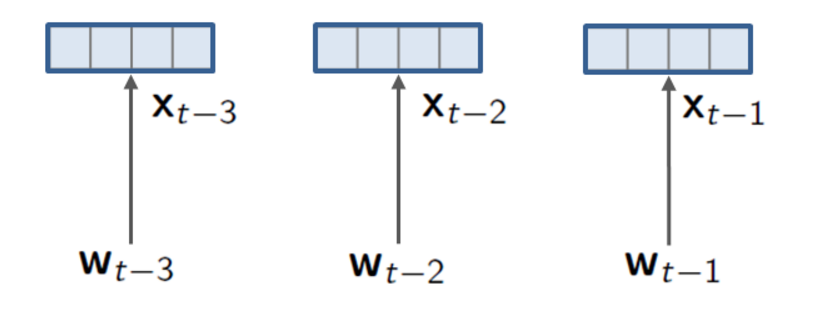
\includegraphics[width=7cm]{emb}
  \end{center}
\end{frame}

% \note{
% So first is the embedding, which maps from an indicator feature to a low-dimension representation. 
% The most common of these has been for word embeddings, which I am sure you have all used. But there
% has also been interesting work on other feature embeddings for tasks like dependency parsing.  
% }

\begin{frame}
  \vspace{-5cm}
  
  \hspace*{-2cm}
  \includegraphics[width=1.5\textwidth]{graph}
\end{frame}


% \begin{frame}

%   \begin{center}
%     \begin{tabular}{cclll}
%       % \structure{Embeddings} & & sparse features &$\Rightarrow$& dense features \\\\
%       \structure{Convolutions} &&  feature n-grams & $\Rightarrow$& dense features  \\\\
%       % \structure{RNNs} & & feature sequences & $\Rightarrow$ &dense features \\
%     \end{tabular}
%   \end{center}

%   \begin{center}
%     \includegraphics[width=9cm]{conv}
%   \end{center}

% \end{frame}

% \begin{frame}
%   \air 

%   \includegraphics[width=\textwidth,trim={0 0 0 19.5cm},clip]{filters}

%   \begin{center}
%     \Cite{DBLP:conf/eccv/ZeilerF14}
%   \end{center}
% \end{frame}

% \begin{frame}
%   \begin{center}
%     \includegraphics[width=9cm]{alpha}
%   \end{center}

%   \begin{center}
%     \Cite{silver2016mastering}
%   \end{center}
% \end{frame}


\begin{frame}
  \begin{center}
    \begin{tabular}{cclll}
      \structure{RNNs/LSTMs} & & feature sequences & $\Rightarrow$ &dense features \\\\
    \end{tabular}
  \end{center}


  \begin{center}
    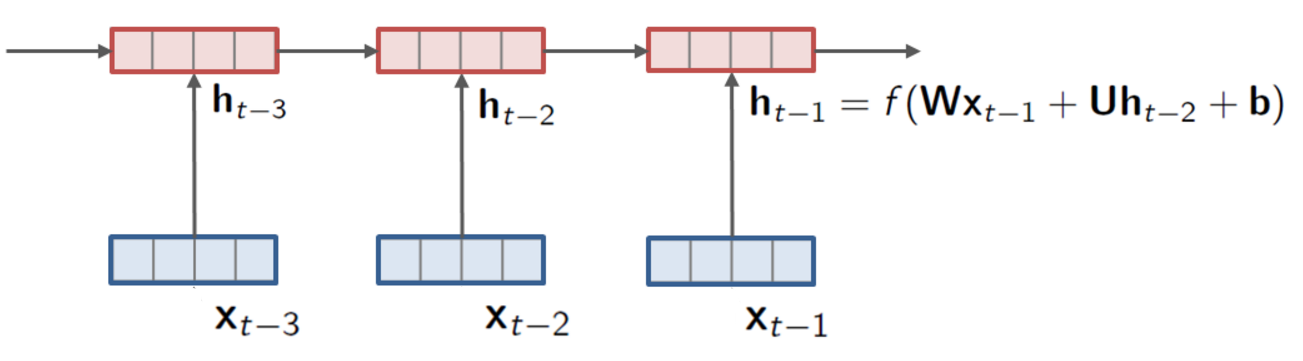
\includegraphics[width=11cm]{rnn}
  \end{center}

  % (In practice, LSTM update semantics are used for all these applications.)
  % \begin{itemize}
  % \item 
  % \end{itemize}
  
\end{frame}


% % \begin{frame}
% %     \includegraphics[width=\textwidth]{good}
% %     \caption{Xu et al (2015)}  
% % \end{frame}

\begin{frame}
  \begin{center}
    \begin{tabular}{cclll}
      \structure{Softmax} & & dense features & $\Rightarrow$ & discrete predictions \
    \end{tabular}
    \air 

    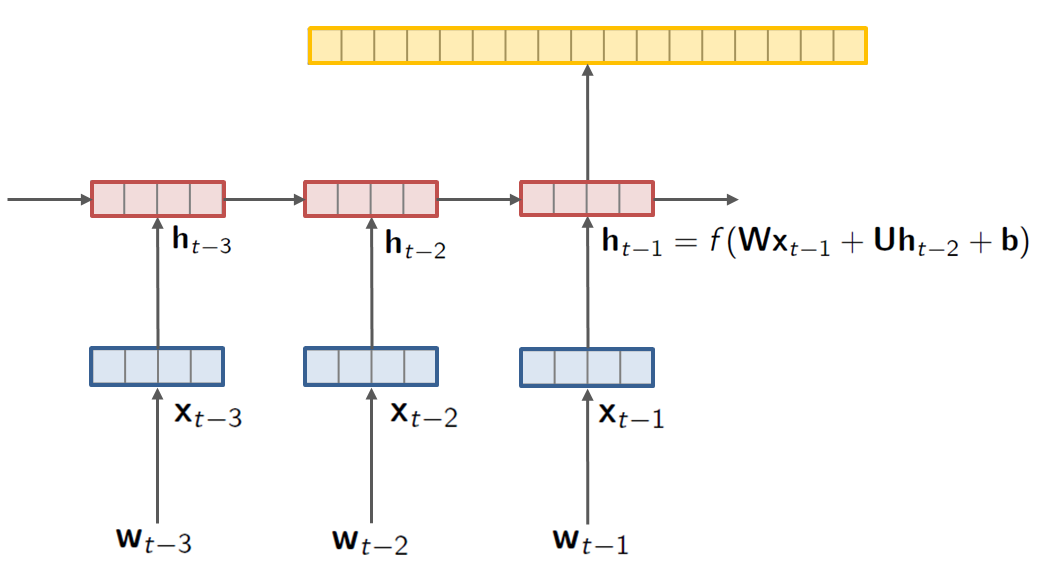
\includegraphics[width=0.8\textwidth]{rnnlm5}
  \end{center}
  \[ p(\wvec_t | \wvec_1, \ldots, \wvec_{t-1}; \theta) = \text{softmax}(\mathbf{W}_{out} \mathbf{h}_{t-1} + \mathbf{b}_{out}) \] 

  \[ p(\wvec_{1:T} ) = \prod_{t} p(\wvec_t | \wvec_1, \ldots, \wvec_{t-1}) \] 
    % \caption{Xu et al (2015)}  
\end{frame}


\begin{frame}
  \begin{center}
    \structure{Contextual Language Model / ``seq2seq''}
  \end{center}
    \air 
   
    \begin{center}
      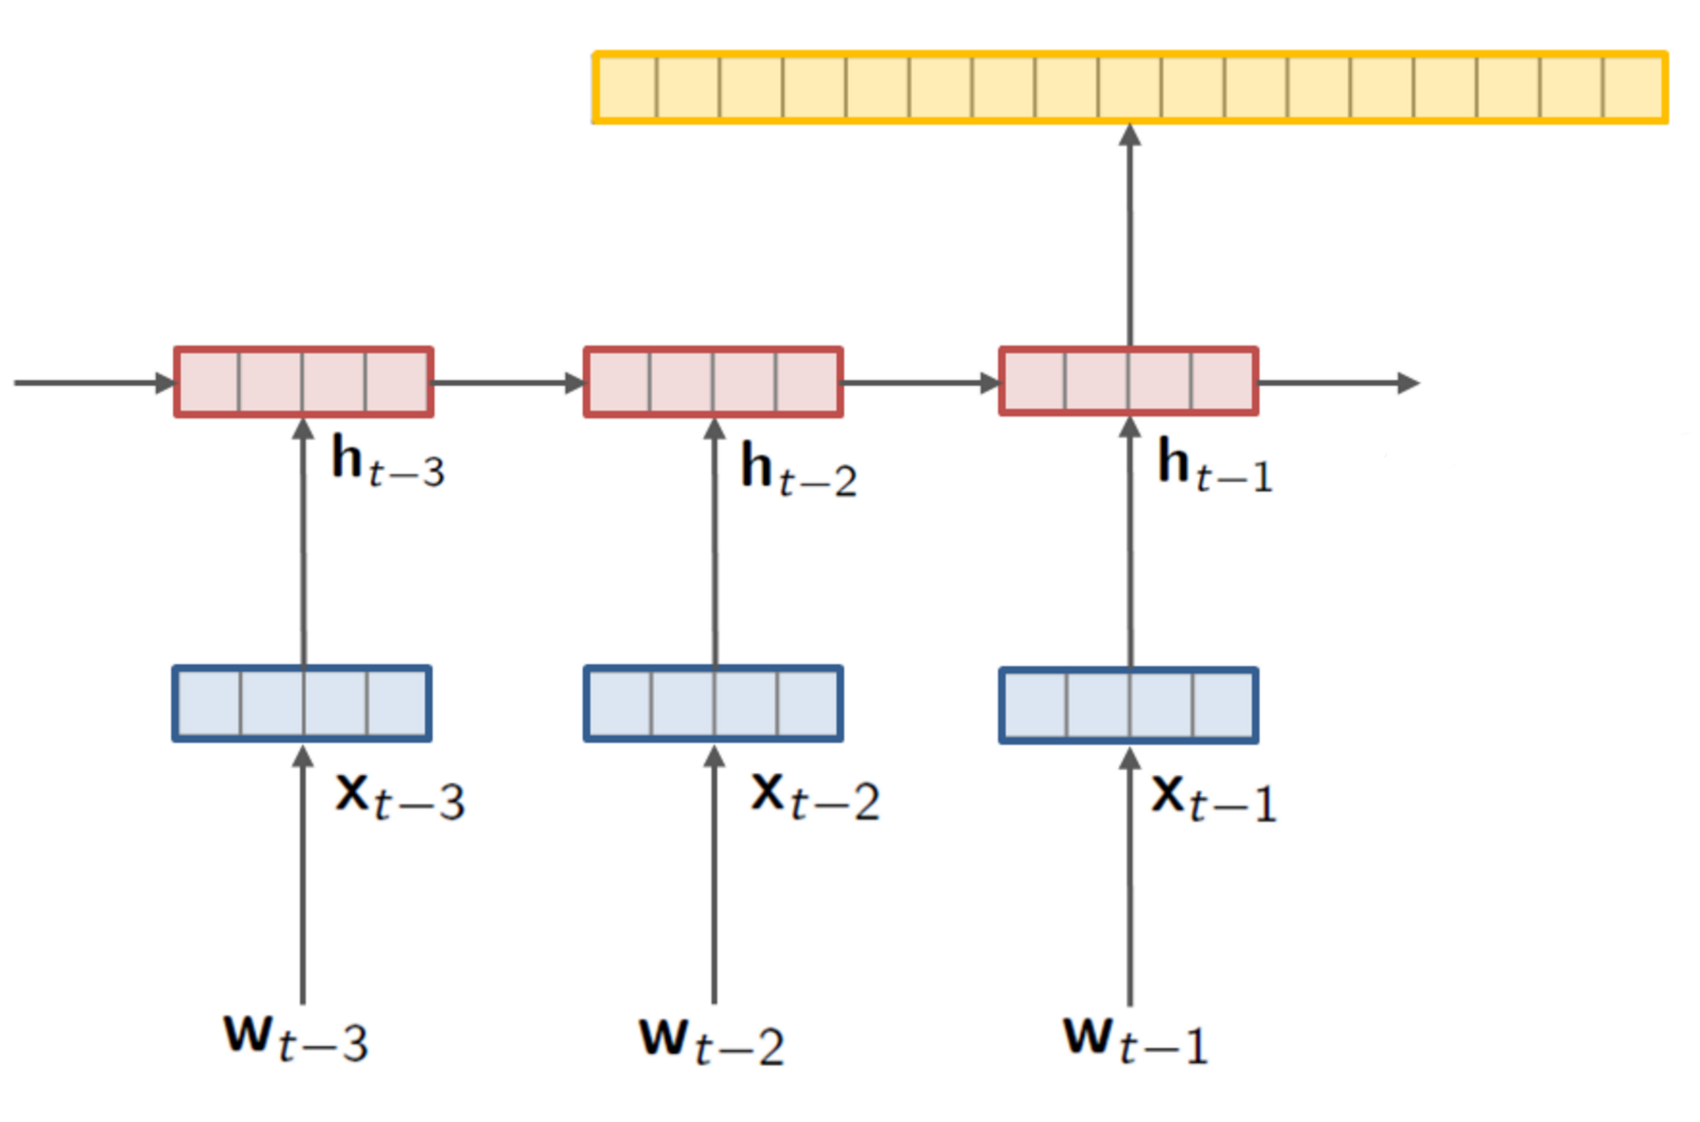
\includegraphics[width=0.6\textwidth]{rnnlm6}
    \end{center}
  \begin{itemize}
  \item Key idea, contextual language model based on encoder $\cvec$: 
  \end{itemize}
  \[ p(\wvec_{1:T} | \cvec) = \prod_{t} p(\wvec_t | \wvec_1, \ldots, \wvec_{t-1}, \cvec) \] 
  
\end{frame}


\begin{frame}
  \begin{center}
    Actual Seq2Seq / Encoder-Decoder / Attention-Based Models
  \end{center}
    \begin{center}
      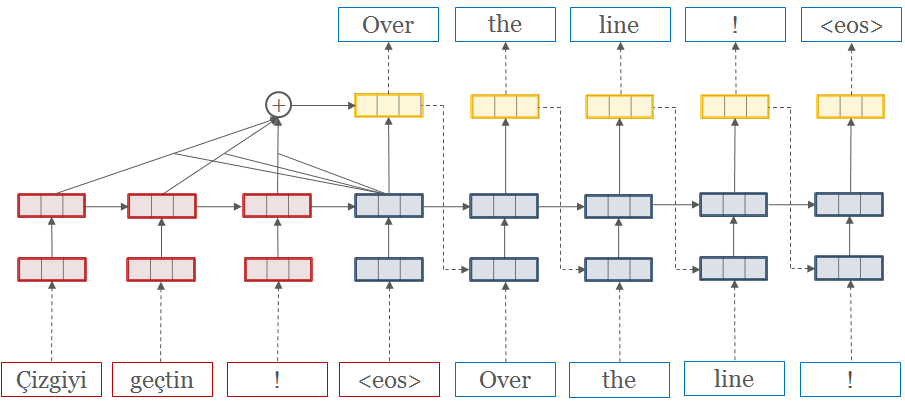
\includegraphics[width=0.7\textwidth]{simple-attn}
    \end{center}
  \begin{itemize}
  \item Different encoders, attention mechanisms, input feeding, ...
    \air
  \item Almost all models use LSTMs or other gated RNNs 
    \air
  \item Large multi-layer networks  necessary for good performance.
    \begin{itemize}
    \item 4 layer, 1000 hidden dims is common for MT
    \end{itemize}
  % \item Main idea, contextual language model based on encoder $\cvec$: 
  \end{itemize}
  % \[ p(\wvec_{1:T} | \cvec) = \prod_{t} p(\wvec_t | \wvec_1, \ldots, \wvec_{t-1}, \cvec) \] 
\end{frame}

\begin{frame}
  \centerline{\textbf{Seq2Seq Applications:} \alert{Sentence Summarization} \Cite{Rush2015} }
  \begin{center}
    \textbf{Source}
  \end{center}
  
  \begin{figure}
    \textit{\structure{Russian Defense Minister Ivanov}
      called \structure{Sunday} for the creation of
      a joint front \structure{for combating} global terrorism. }
  \end{figure}

  \begin{center}
    \textbf{Target}
  \end{center}
  \mair

  \begin{figure}
    \centering
    \textit{\structure{Russia} calls for joint
      front \structure{against} terrorism.}
  \end{figure}

\air
\air


% \textbf{Summarization Phenomena:} 

% \begin{itemize}
% \item<2-> \alert<2>{Generalization}
% \item<3-> \alert<3>{Deletion}
% \item<4-> \alert<4>{Paraphrase}
% % \item<5-> \alert<5>{Tense}
% \end{itemize}
\pause
  \begin{itemize}
  \item Used by The Washington Post to suggest headlines \Cite{shuguangwang}
  \end{itemize}
\end{frame}

\begin{frame}
  \centerline{\textbf{Seq2Seq Applications:} \alert{Grammar Correction} \Cite{Schmaltz2016} }
  % \centerline{\structure{Grammar Correction} \cite{}}
  
  \begin{center}
    \textbf{Source}
  \end{center}
  
  \begin{figure}
    \textit{There is no \structure{a doubt}, tracking \structure{systems has} brought many benefits in this information
age . }
  \end{figure}

  \begin{center}
    \textbf{Target}
  \end{center}
  \mair

  \begin{figure}
    \centering
    \textit{There is no doubt, tracking systems have
      brought many benefits in this information
      age . }
  \end{figure}
  \pause

  \begin{itemize}
  \item First-place on BEA 11 grammar correction shared task \Cite{Daudaravicius2016}
  \end{itemize}
\end{frame}


\begin{frame}
  \centerline{\structure{This Talk}}
  \air 
  \air

  \begin{itemize}
  \item How can we \textbf{interpret} these learned hidden representations? 
    \air 

    

  \item  How should we \textbf{train} these style of models? 
    \air 
  \item  How can we \textbf{shrink} these models for practical applications? 
  \end{itemize}
\end{frame}

\begin{frame}
  \centerline{\structure{This Talk}}
  \air 
  \air

  \begin{itemize}
  \item How can we \textbf{interpret} these learned hidden representations? 

    \begin{center}
      \alert{LSTMVis} 

      \Cite{Strobelt2016}
    \end{center}


    \air 

    

  \item  \textcolor{gray}{How should we \textbf{train} these style of models? \Cite{Wiseman2016a}}
    \air 
  \item  \textcolor{gray}{How can we \textbf{shrink} these models for practical applications? \Cite{Kim2016a}}
  \end{itemize}
\end{frame}


\section{Interpretation}

\begin{frame}
  \air 
  \includegraphics[width=\textwidth,trim={0 0 0 19.5cm},clip]{filters}
  \begin{center}
     \Cite{DBLP:conf/eccv/ZeilerF14}
  \end{center}
\end{frame}

% \begin{frame}
%   \begin{frame}
%   \begin{center}
%     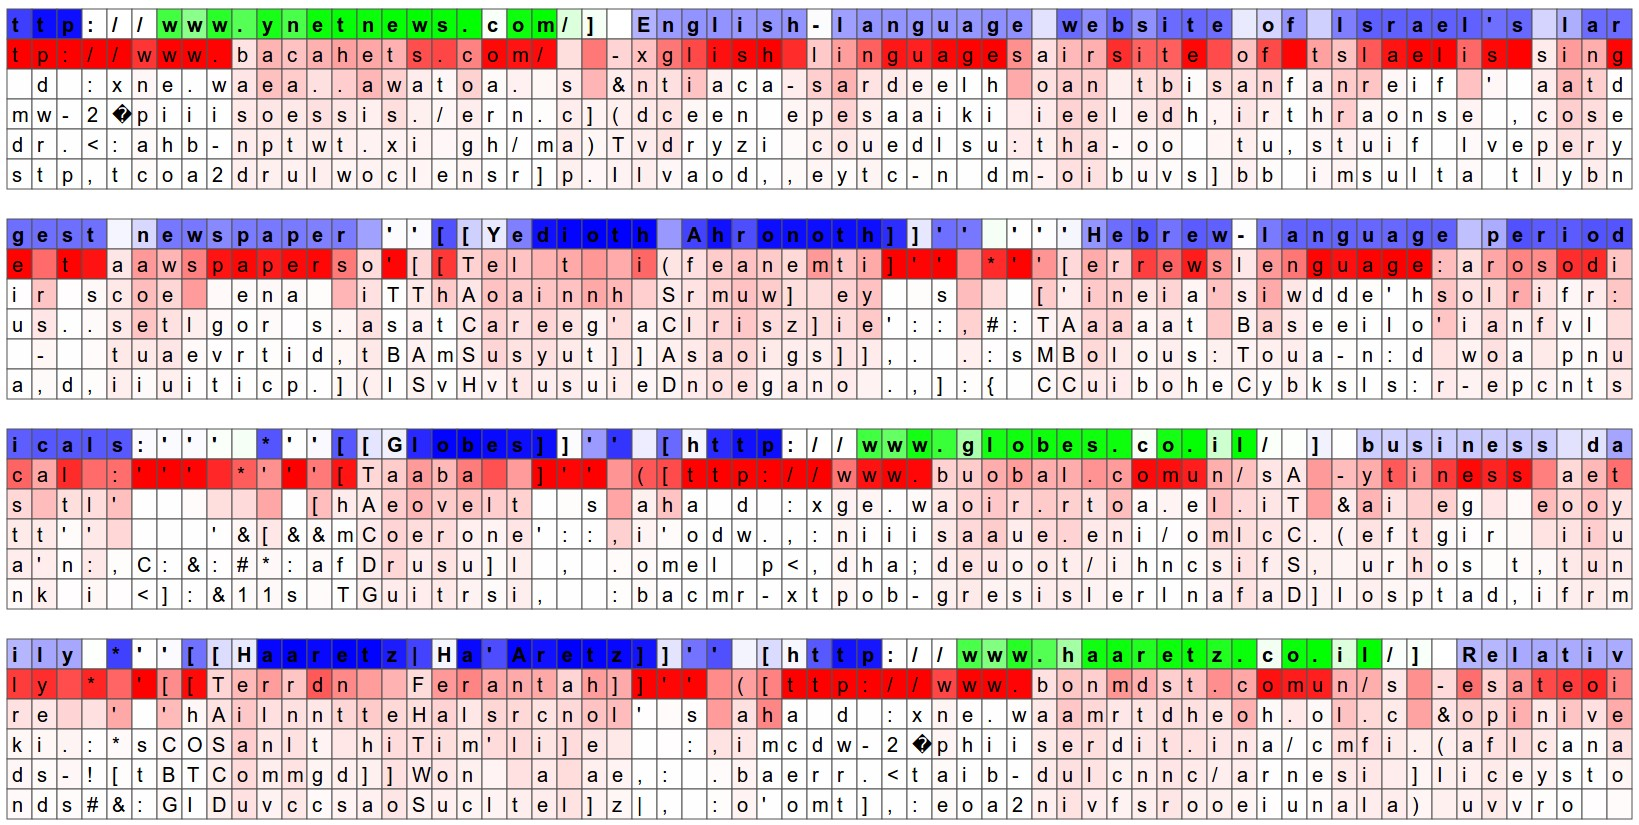
\includegraphics[width=\textwidth]{lstm1}

%     {\footnotesize (Karpathy et al, 2015)}
%   \end{center}

%     % \caption{Xu et al (2015)}  
% \end{frame}


\begin{frame}
  % \begin{frame}
  \centerline{Vector-Space RNN Representation}
  \begin{center}
    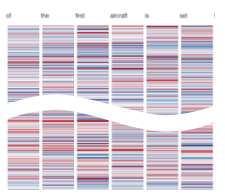
\includegraphics[height=5cm]{lstmrep}
  \begin{center}
    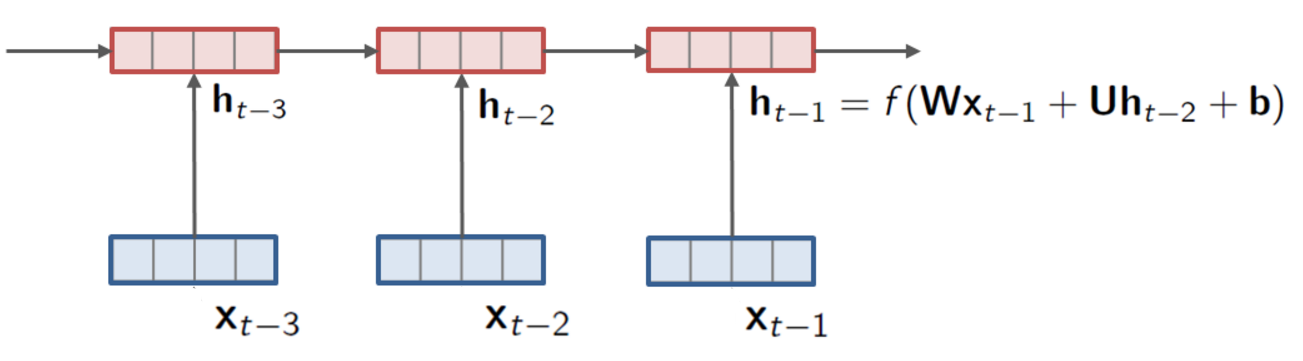
\includegraphics[width=11cm]{rnn}
  \end{center}


  \end{center}
\end{frame}


\begin{frame}
  % \begin{frame}
  \begin{center}
    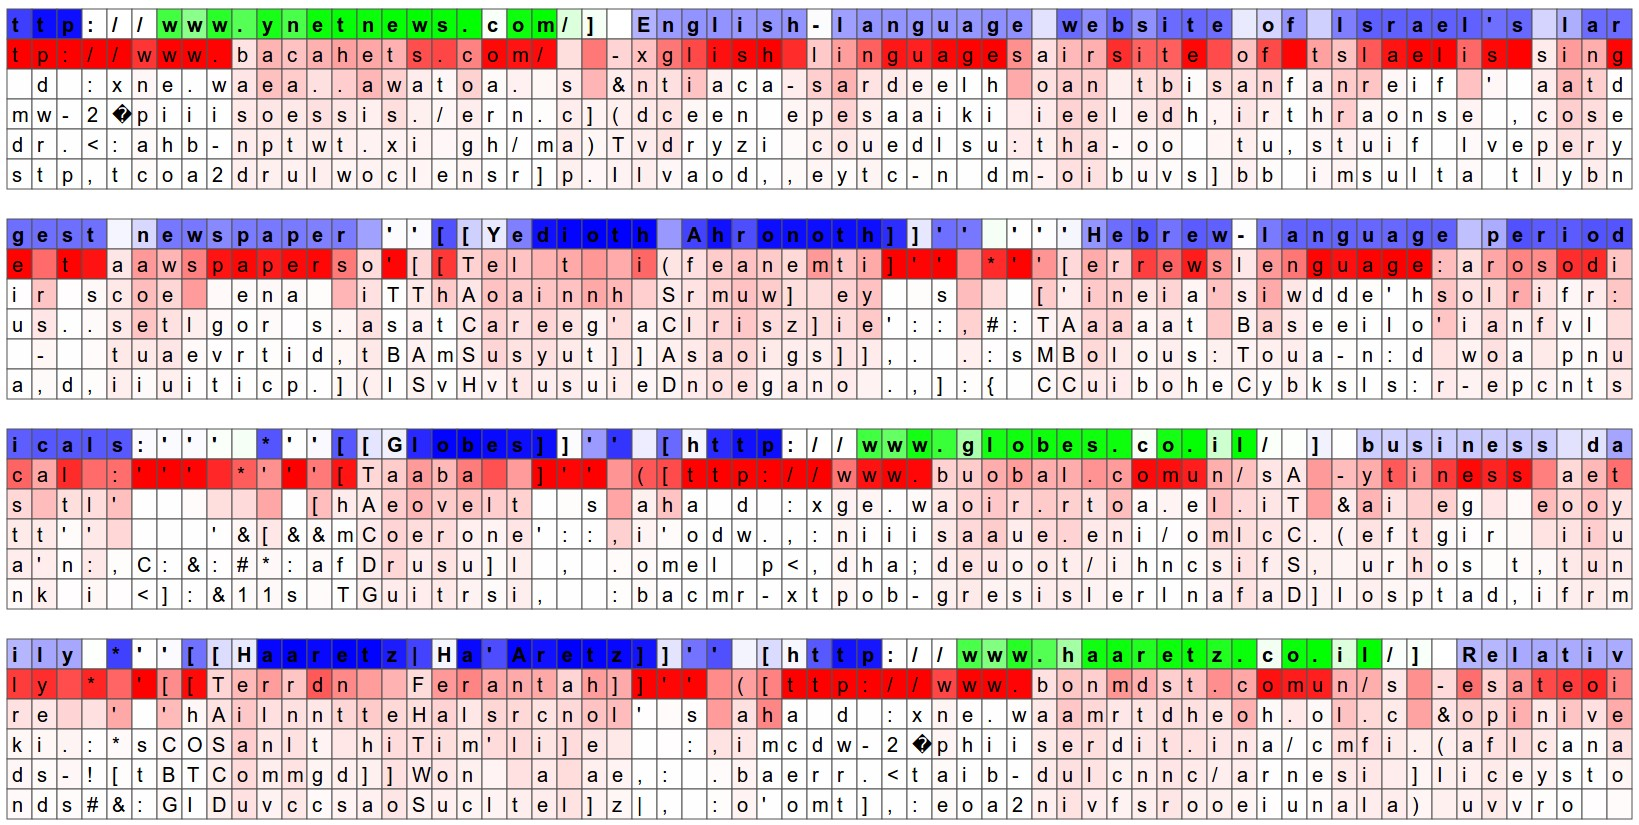
\includegraphics[width=\textwidth]{lstm1}

     \Cite{karpathy2015visualizing}
    % {\footnotesize (Karpathy et al, 2015)}
  \end{center}
    % \caption{Xu et al (2015)}  
\end{frame}

\begin{frame}
  \centerline{\alert{Example 1}: Synthetic (Finite-State) Language}
  \air

  \begin{center}
    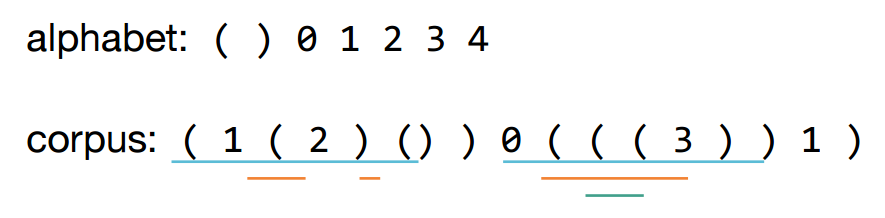
\includegraphics[width=9cm]{parenlang}
  \end{center}
  \mair

  \begin{itemize}
  \item Numbers are randomly generated, must match nesting level.
    \air

  \item Train a predict-next-word language model (decoder-only).
  \end{itemize}
    \[ p(\wvec_t | \wvec_1, \ldots, \wvec_{t-1}) \] 
  
\air
  \centerline{\href{http://lstm.seas.harvard.edu/client/pattern_finder.html?data_set=00parens&source=states::states2&pos=150}{[Parens Example]}}
\end{frame}


\begin{frame}
  \centerline{\alert{Example 2}: Real Language}
  \air

  \begin{description}
  \item[alphabet:] all english words
  \item[corpus:] Project Gutenberg Children's books 
  \end{description}
  % \begin{center}
  %   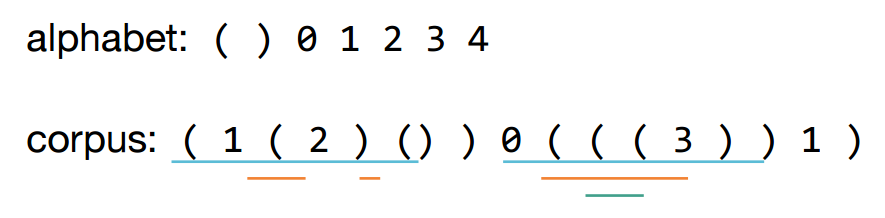
\includegraphics[width=9cm]{parenlang}
  % \end{center}

  \begin{itemize}
  % \item 
  %   \air

  \item Train a predict-next-word language model (decoder-only).

  
  \end{itemize}
    \[ p(\wvec_t | \wvec_1, \ldots, \wvec_{t-1}) \] 

\air
  \centerline{ \href{http://lstm.seas.harvard.edu/client/pattern_finder.html?data_set=05childbook&source=states::states1&pos=100}{[LM Example]}}
\end{frame}


\begin{frame}
  \centerline{\alert{Example 3}: Seq2Seq Encoder}
  \air

  \begin{description}
  \item[alphabet:] all english words
  \item[corpus:]  Summarization
  \end{description}
  % \begin{center}
  %   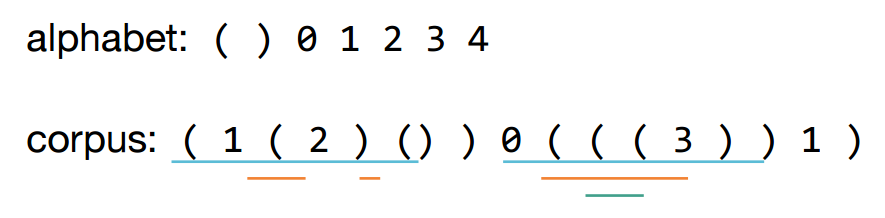
\includegraphics[width=9cm]{parenlang}
  % \end{center}

  \begin{itemize}
  % \item 
  %   \air

  \item Train a full seq2seq model, examine \textit{encoder} LSTM.
  
  \end{itemize}


\air
  \centerline{ \href{http://lstm.seas.harvard.edu/client/pattern_finder.html?data_set=20autoencoder&source=states::states2&pos=100}{[Summarization Example]}}
\end{frame}

% \begin{frame}
%   \centerline{LSTMVis: Next Steps}

%   \begin{itemize}
%   \item More models
%     \air

%   \item Further data annotations
%     \air
%   \item 
      
%   \end{itemize}

%   % \begin{center}
%   %   \includegraphics{}
%   % \end{center}
%   \begin{itemize}
%   \item 
%   \end{itemize}
% \end{frame}

\begin{frame}
  \centerline{\structure{This Talk}}
  \air 
  \air

  \begin{itemize}
  \item \textcolor{gray}{How can we \textbf{interpret} these learned hidden representations? \Cite{Strobelt2016}}
    \air 
  \item  How should we \textbf{train} these style of models? 
    \air 

    \begin{center}
      \alert{Sequence-to-Sequence Learning as Beam-Search
        Optimization}

      \Cite{Wiseman2016a}
    \end{center}


    \air 
  \item \textcolor{gray}{ How can we \textbf{shrink} these models for practical applications \Cite{Kim2016a}? }
  \end{itemize}
\end{frame}

\begin{frame}
  \centerline{Some More Seq2Seq \alert{Details} }
  \air 
  \air

  Training Objective: Multiclass NLL (for training targets $y_{1:T}$)
  \[ \text{NLL}(\theta) = -\sum_{t} \log p(\wvec_{t} = y_t | \wvec_{1:t-1} = y_{1:t-1}, \cvec; \theta) \] 

  \air

  Test Objective: Structured output space

  \[ \wvec^*_{1:T} = \argmax_{\wvec_{1:T}} \sum_{t} \log p(\wvec_{t} | \wvec_{1:t-1}, \cvec; \theta) \] 
  \pause
  \begin{itemize}
  \item Note: Completely intractable $O(\text{\#vocab} ^T)$ 
  \end{itemize}
\end{frame}

\begin{frame}
  \centerline{Standard Approach: \structure{Beam Search}}
  \air 


  \begin{enumerate}
  \item Start with $K$ partial starting hypotheses $\wvec^{(1:K)}$
  \item For timesteps $t$ from  $1$ to $T$:
    \pause
   \begin{enumerate}
   \item Compute for all $k, \wvec_{t}$
     \[s(\wvec_t, \wvec_{1:t-1}^{(k)}) \gets \log p(\wvec_{t} | \wvec^{(k)}_{1:t-1}, \cvec) + \log p(\wvec^{(k)}_{1:t-1}| \cvec) \]
    \pause
   \item Replace the $K$ highest scoring target sequences
     \[\wvec_{1:t}^{(1:K)} \gets K\argmax_{\wvec_{1:t}} s(\wvec_t, \wvec_{1:t-1}^{(k)})\]  
   \end{enumerate}
  \end{enumerate}


  % \begin{enumerate}
  % \item Start with $K$ partial starting hypotheses $\wvec^{(1:K)}$
  % \item For timesteps $t$ from  $1$ to $T$:
  %  \begin{enumerate}
  %  \item Compute for all $k, \wvec_{t}$
  %    \[s(\wvec_t, k) \gets \log p(\wvec_{t} | \wvec^{(k)}_{1:t-1}, \cvec; \theta) + \log p(\wvec^{(k)}_{1:t-1}| \cvec;\theta) \]
  %  \item Save $K$ highest scoring target sequences
  %    \[\wvec_{1:t+1}^{(1:K)} \gets K\arg\max_{\wvec_t, k} s(\wvec_t, k)\]  
  %  \end{enumerate}
  % \end{enumerate}
  \pause
  % \begin{itemize}
  % \item Note: Requires computing $p(\wvec_{t} | \wvec^{(k)}_{1:t-1}, \cvec; \theta)$ for many  $\wvec^{(k)}_{1:t-1}$ 
  % \end{itemize}
\end{frame}

\begin{frame}[fragile]
    \begin{center}
      \structure{Beam Search Example} ($K=3$)
    \end{center}
    \air
    \air
   \air
  
    \begin{center}
  \begin{tikzpicture}[transform canvas = {scale=0.8}]
    \tikzstyle{beam}=[draw, minimum height=0.6cm, anchor=base, text height=5, text depth=0, minimum width=1.5cm,thin, rounded corners, line width=0.03cm]
   \tikzstyle{mat}=[draw=white]
    \tikzset{>=stealth',every on chain/.append style={join},
      every join/.style={->}}

     
       \begin{scope}
         
   \matrix (G) [matrix of nodes, nodes={beam},inner sep=1mm,row sep=0.03cm, column sep=0.8cm ] {
    \node<1->(G-1-1){a}; & \node<2->(G-1-2){red}; & \node<3->(G-1-3){dog}; & \node<4->(G-1-4){smells}; & \node<5->(G-1-5){home};  & \node<6->(G-1-6){today}; \\
    \node<1->(G-2-1){the}; & \node<2->(G-2-2){dog}; & \node<3->(G-2-3){dog}; & \node<4->(G-2-4){barks}; & \node<5->(G-2-5){quickly}; & \node<6->(G-2-6){Friday}; \\
    \node<1->(G-3-1){red}; & \node<2->(G-3-2){blue}; & \node<3->(G-3-3){cat}; &  \node<4->(G-3-4){barks}; & \node<5->(G-3-5){straight}; & \node<6->(G-3-6){now}; \\    };

    \only<2->{
      \draw[->] (G-1-1.east) -> (G-1-2.west); 
      \draw[->] (G-2-1.east) -> (G-2-2.west); 
      \draw[->] (G-1-1.east) -> (G-3-2.west); 
      \draw[double, line width=0.03cm] (G-3-1.south west) -- (G-3-2.south east);
    }
  
    \only<3->{
      \draw[->] (G-1-2.east) -> (G-2-3.west); 
      \draw[->] (G-3-2.east) -> (G-3-3.west); 
      \draw[->] (G-3-2.east) -> (G-1-3.west); 
      \draw[double, line width=0.03cm] (G-3-1.south west) -- (G-3-3.south east);
    }
    
 \only<4->{
    \draw[->] (G-1-3.east) -> (G-3-4.west); 
    \draw[->] (G-2-3.east) -> (G-2-4.west); 
    \draw[->] (G-1-3.east) -> (G-1-4.west); 
    \draw[double, line width=0.03cm] (G-3-1.south west) -- (G-3-4.south east);
}
 \only<6->{
    \draw[->] (G-1-5.east) -> (G-1-6.west); 
    \draw[->] (G-1-5.east) -> (G-3-6.west); 
    \draw[->] (G-2-5.east) -> (G-2-6.west); 
    \draw[double, line width=0.03cm] (G-3-1.south west) -- (G-3-6.south east);
}

 \only<5->{
    \draw[->] (G-3-4.east) -> (G-1-5.west); 
    \draw[->] (G-3-4.east) -> (G-2-5.west); 
    \draw[->] (G-3-4.east) -> (G-3-5.west); 
    \draw[double, line width=0.03cm] (G-3-1.south west) -- (G-3-5.south east);
}

\end{scope}
\end{tikzpicture}
    \end{center}
    \air

For timesteps $t$ from  $1$ to $T$:
   \begin{enumerate}
   \item Compute for all $k, \wvec_{t}$
     \[s(\wvec_t, \wvec_{1:t-1}^{(k)}) \gets \log p(\wvec_{t} | \wvec^{(k)}_{1:t-1}, \cvec) + \log p(\wvec^{(k)}_{1:t-1}| \cvec) \]
   \item Replace the $K$ highest scoring target sequences
     \[\wvec_{1:t}^{(1:K)} \gets K\argmax_{\wvec_{1:t}} s(\wvec_t, \wvec_{1:t-1}^{(k)})\]  
   \end{enumerate}

\end{frame}

\begin{frame}
  \centerline{Theoretical \alert{Issues} with Standard Setup}
  \begin{itemize}

  \item Exposure Bias
    \begin{itemize}
    \item Training by conditioning on true $y_{1:t-1}$, 
      \[ p(\wvec_{t} = y_t | \wvec_{1:t-1} = y_{1:t-1}, \cvec; \theta)\]
    \end{itemize}
    \air
  \item Train/Test Loss Mismatch 
    \begin{itemize}
    \item Training with local NLL, evaluate with hamming-style losses (BLEU)  
    \end{itemize}

    \air
  \item Label Bias  \Cite{Lafferty2001}
    \begin{itemize}
    \item Locally normalized models have known pathological issues
    \end{itemize}

  \end{itemize}
\end{frame}

\begin{frame}
  \centerline{\structure{Related Work:} Modify training data}
  \air 
  \begin{itemize}
  \item Data as Demonstrator \Cite{Venkatraman}, Scheduled Sampling \Cite{Bengio2015}
  \end{itemize}
  \air 

  \centerline{\structure{Related Work:} Use Reinforcement Learning}
  \air 
  \begin{itemize}
  \item MIXER \Cite{Ranzato2016}
  \item Actor-Critic \Cite{Bahdanau2016}
  \end{itemize}
  
  \pause

  Opinion: 
  \begin{itemize}
  \item 
    DAD methods only address exposure bias, 
  \item RL is too strong a hammer .
  \end{itemize}

  % \begin{itemize}
  % \item 
  % \end{itemize}
\end{frame}


\begin{frame}
  \begin{center}
    Our Proposal: \structure{Seq2Seq as Beam Search Optimization}
  \end{center}

  New Setup: Run beam search at training. 
  \air 

  
  \begin{itemize}

  \item (Idea 1) Replace local softmax with sequence scorer $f$
    \air 
  \item (Idea 2) Run beam search during training time 
    \air 

  \item (Idea 3) Replace local training objective with beam-search margin
  \end{itemize}
\end{frame}

\begin{frame}
  \begin{center}
    \structure{(Idea 1)} Replace local softmax with sequence scorer $f$
    \air 

    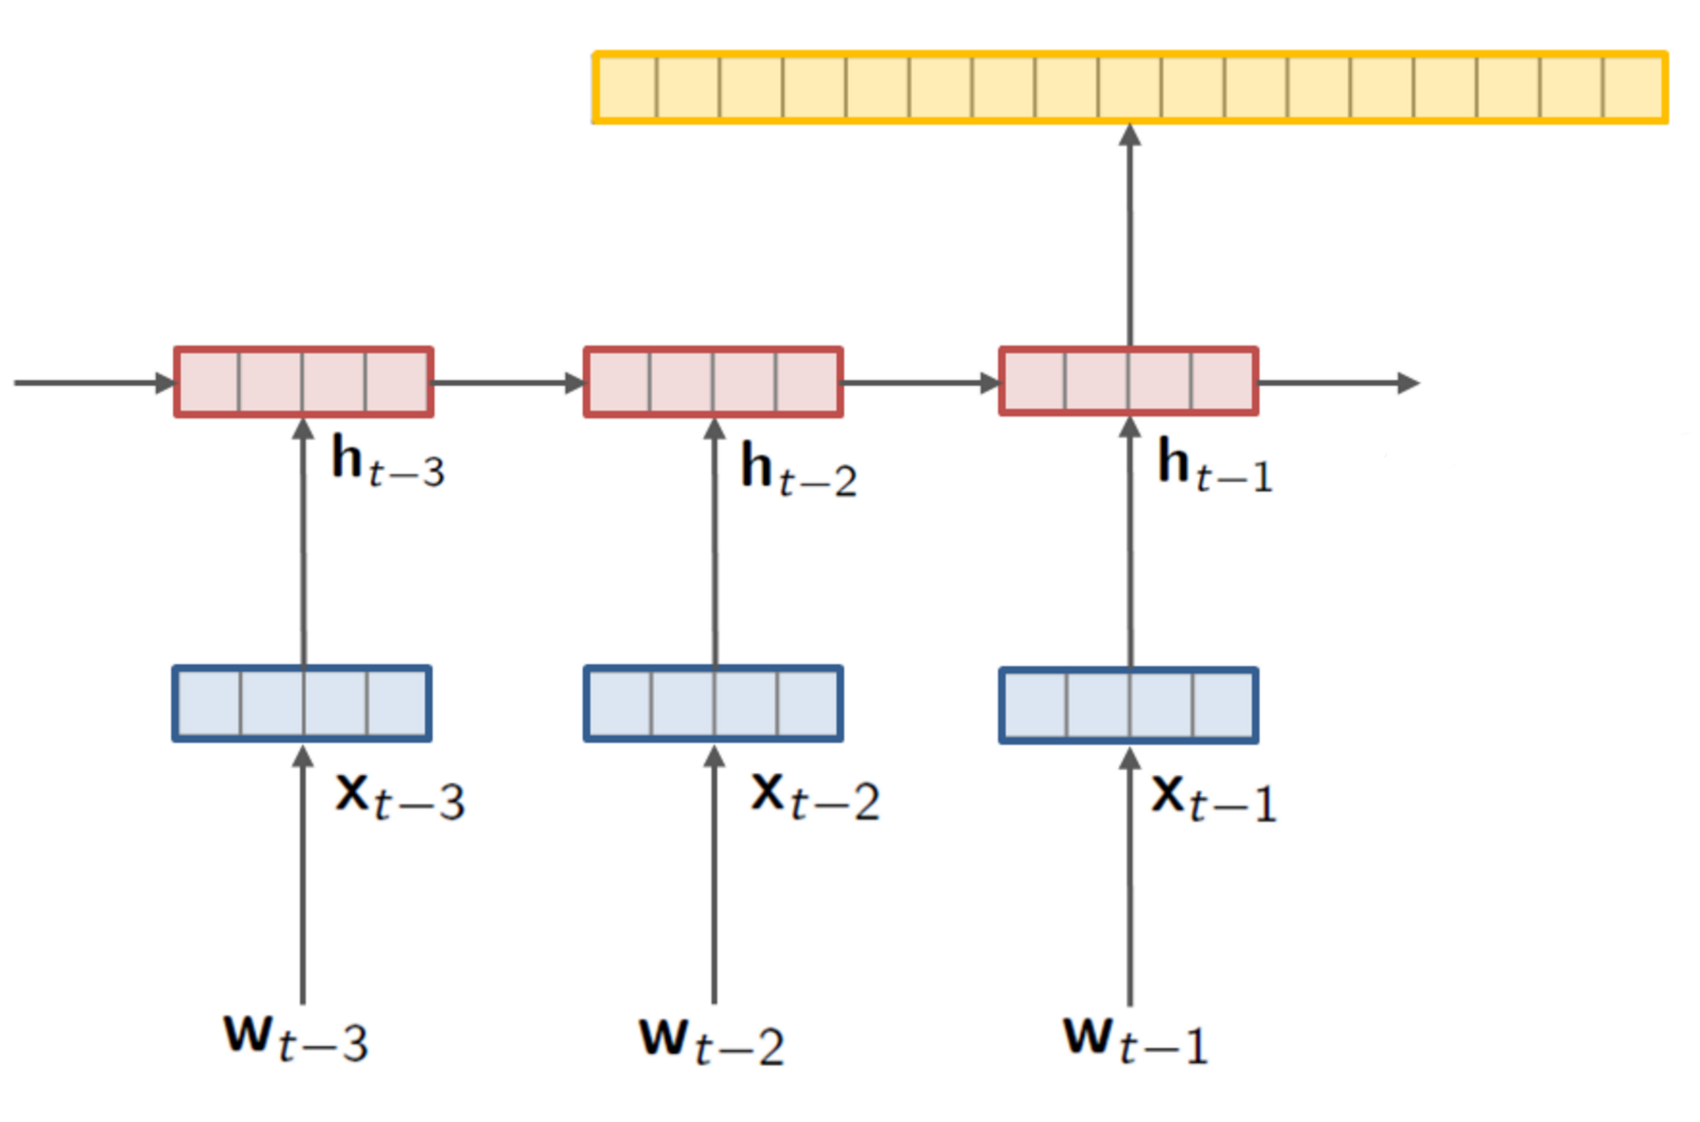
\includegraphics[width=0.6\textwidth]{rnnlm6}
  \end{center}

  Same model, but replace 
  $  \log p(\wvec_{t} | \wvec^{(k)}_{1:t-1}, \cvec; \theta)$
  with unnormalized 
  $f(\wvec_t, \wvec_{1:t-1}^{(k)}, \cvec; \theta)$
\end{frame}

\begin{frame}
  \begin{center}
    \structure{(Idea 2)} Run beam search during training
  \end{center}
  \begin{enumerate}
  \item Start with $K$ partial starting hypotheses $\wvec^{(1:K)}$
  \item For timesteps $t$ from  $1$ to $T$:
   \begin{enumerate}
   \item Compute for all $k, \wvec_{t}$
     \only<1>{
     \[s(\wvec_t, \wvec_{1:t-1}^{(k)}) \gets \alert{\log p(\wvec_{t} | \wvec^{(k)}_{1:t-1}, \cvec; \theta) + \log p(\wvec^{(k)}_{1:t-1}| \cvec;\theta)} \]
   }
   \only<2>{
     \[s(\wvec_t, \wvec_{1:t-1}^{(k)})  \gets  \structure{f(\wvec_t, \wvec_{1:t-1}^{(k)}, \cvec; \theta)} \]
   }
   \item Replace the  $K$ highest scoring target sequences
     \[\wvec_{1:t}^{(1:K)} \gets K\argmax_{\wvec_{1:t}} s(\wvec_t, \wvec_{1:t-1}^{(k)})\]  
   \end{enumerate}
  \end{enumerate}

\end{frame}


\begin{frame}
  \begin{center}
    \structure{(Idea 3)} Replace local training objective with beam-search margin 
  \end{center}

  New Objective: 
  \begin{itemize}

  \item Margin between target seq $y$ and last seq on beam $\wvec^{(K)}$  
  \end{itemize}
\begin{align*}
 \mathcal{L}&(\theta) = \sum_{t} \Delta(y_{1:t}, \wvec_{1:t}^{K}) \left[1 - f(y_t, y_{1:t-1}, \cvec) +  f(\wvec_t^{(K)}, \wvec_{1:t-1}^{(K)}, \cvec) \right] 
\end{align*}

\begin{itemize}
  \item Slack-rescaled, margin-based sequence criterion, at each time step.  
\item When violation occurs, target replaces current beam (learning as search optimization \Cite{daume05learning})
\end{itemize}

\end{frame}

\begin{frame}[fragile]
  \begin{center}
    \begin{center}
      Beam Search Optimization Example ($K=3$)
    \end{center}
    \air
    \air
    \air
    \air

  \begin{tikzpicture}[transform canvas = {scale=0.8}]
  \tikzstyle{beam}=[draw, minimum height=0.6cm, anchor=base, text height=5, text depth=0, minimum width=1.5cm,thin, rounded corners, line width=0.03cm]
  \tikzstyle{mat}=[draw=white]
\tikzset{>=stealth',every on chain/.append style={join},
         every join/.style={->}}

     
       % \node[draw = white, yshift=1.8cm]{Time Step};
       %\node[draw = white, xshift=-7.5cm, yshift=0.5cm]{Beam:};
       \begin{scope}
         

   \matrix (G) [matrix of nodes, nodes={beam},inner sep=1mm,row sep=0.03cm, column sep=0.8cm ] {
    \node<1->[fill=yellow](G-1-1){\textcolor{blue}{a}}; & \node<2->[fill=yellow](G-1-2){red}; & \node<3->[fill=lightgray](G-1-3){\textcolor{blue}{dog}}; & \node<4->(G-1-4){smells}; & \node<5->[fill=lightgray](G-1-5){\textcolor{red}{home}};  & \node<6->[fill=lightgray](G-1-6){\textcolor{red}{today}}; \\
    \node<1->(G-2-1){the}; & \node<2->(G-2-2){dog}; & \node<3->[fill=yellow](G-2-3){dog}; & \node<4->(G-2-4){barks}; & \node<5->[fill=yellow](G-2-5){quickly}; & \node<6->(G-2-6){Friday}; \\
    \node<1->(G-3-1){red}; & \node<2->[fill=lightgray](G-3-2){\textcolor{blue}{blue}}; & \node<3->(G-3-3){cat}; &  \node<4->[fill=lightgray](G-3-4){\textcolor{blue}{barks}}; & \node<5->(G-3-5){straight}; & \node<6->[](G-3-6){now}; \\
    & & & \node<4->[fill=yellow](G-4-4){runs}; & & \node<6->[fill=yellow](G-4-6){today}; \\
    };

    \only<2->{
      \draw[->] (G-1-1.east) -> (G-1-2.west); 
      \draw[->] (G-2-1.east) -> (G-2-2.west); 
      \draw[->] (G-1-1.east) -> (G-3-2.west); 
      \draw[double, line width=0.03cm] (G-3-1.south west) -- (G-3-2.south east);
    }
  
    \only<3->{
      \draw[->] (G-1-2.east) -> (G-2-3.west); 
      \draw[->] (G-3-2.east) -> (G-3-3.west); 
      \draw[->] (G-3-2.east) -> (G-1-3.west); 
      \draw[double, line width=0.03cm] (G-3-1.south west) -- (G-3-3.south east);
    }
    
 \only<4->{
    \draw[->] (G-2-3.east) -> (G-4-4.west); 
    \draw[->] (G-1-3.east) -> (G-3-4.west); 
    \draw[->] (G-2-3.east) -> (G-2-4.west); 
    \draw[->] (G-1-3.east) -> (G-1-4.west); 
    \draw[double, line width=0.03cm] (G-3-1.south west) -- (G-3-4.south east);
}
 \only<6->{
    \draw[->] (G-1-5.east) -> (G-1-6.west); 
    \draw[->] (G-1-5.east) -> (G-3-6.west); 
    \draw[->] (G-2-5.east) -> (G-2-6.west); 
    \draw[->] (G-2-5.east) -> (G-4-6.west); 
    \draw[double, line width=0.03cm] (G-3-1.south west) -- (G-3-6.south east);
}

    % \draw[->] (G-3-2.east) -> (G-3-3.west); 
    % \draw[->] (G-3-2.east) -> (G-1-3.west); 

 \only<5->{
    \draw[->, dashed] (G-4-4.east) -> (G-1-5.west); 
    \draw[->, dashed] (G-4-4.east) -> (G-2-5.west); 
    \draw[->, dashed] (G-4-4.east) -> (G-3-5.west); 
    \draw[double, line width=0.03cm] (G-3-1.south west) -- (G-3-5.south east);
}

       \end{scope}
    % \draw(G-1-1.north east) rectangle (G-3-1.south west);
    % \draw(G-1-2.north east) rectangle (G-3-2.south west);

    % \begin{scope}[yshift=-2.8cm]

    %   \matrix (G) [matrix of nodes,nodes={beam}, inner sep=1mm,row sep=0.06cm,column sep=0.8cm ] {
    %     \node[fill=yellow](G-1-1){a}; & \node[fill=yellow](G-1-2){red}; & \node[fill=yellow](G-1-3){dog}; & \node[fill=yellow](G-1-4){runs}; & \node[fill=yellow](G-1-5){quickly}; & \node[fill=yellow](G-1-6){today}; \\
    %      & \node[fill=lightgray](G-2-2){\textcolor{blue}{blue}}; & \node[fill=lightgray](G-2-3){\textcolor{blue}{dog}}; & \node[fill=lightgray](G-2-4){\textcolor{blue}{barks}}; & \node[fill=lightgray](G-2-5){\textcolor{red}{home}}; & \node[fill=lightgray](G-2-6){\textcolor{red}{today}}; \\
    %   };
    % \draw[->] (G-1-1.east) -> (G-1-2.west); 
    % \draw[->] (G-1-2.east) -> (G-1-3.west); 
    % \draw[->] (G-1-3.east) -> (G-1-4.west); 
    % \draw[->] (G-1-4.east) -> (G-1-5.west); 
    % \draw[->] (G-1-5.east) -> (G-1-6.west); 

    % \draw[->] (G-1-1.east) -> (G-2-2.west); 
    % \draw[->] (G-2-2.east) -> (G-2-3.west); 
    % \draw[->] (G-2-3.east) -> (G-2-4.west); 
    % \draw[->] (G-1-4.east) -> (G-2-5.west); 
    % \draw[->] (G-2-5.east) -> (G-2-6.west); 
      
    % \end{scope}
\end{tikzpicture}
  \end{center}  

  \air 
  \air 
% \begin{align*}
%  \mathcal{L}&(\theta) = \sum_{t} \Delta(\wvec_{1:t}, \wvec_{1:t}^{(K)}) \left[1 - f(\wvec_t, \wvec_{1:t-1}, \cvec) +  f(\wvec_t^{(K)}, \wvec_{1:t-1}^{(K)}, \cvec) \right] 
% \end{align*}

  \begin{itemize}
  \item Color \textcolor{yellow}{Gold}: target sequence $y$
  \item Color \textcolor{gray}{Gray}: violating sequence $\wvec^{(K)}$
  \end{itemize}
\end{frame}

\begin{frame}[fragile]
  \centerline{Structured Backpropagation}
  \begin{center}
    
  \air 
  \air 
  \air 

  \begin{tikzpicture}[transform canvas = {scale=0.8}]
    \tikzstyle{beam}=[draw, minimum height=0.6cm, anchor=base, text height=5, text depth=0, minimum width=1.5cm,thin, rounded corners, line width=0.03cm]
    \tikzstyle{mat}=[draw=white]
    \tikzset{>=stealth',every on chain/.append style={join},
      every join/.style={->}}
    
     
       % \node[draw = white, yshift=1.8cm]{Time Step};
       %\node[draw = white, xshift=-7.5cm, yshift=0.5cm]{Beam:};
       \begin{scope}
         

   \matrix (G) [matrix of nodes, nodes={beam},inner sep=1mm,row sep=0.03cm, column sep=0.8cm ] {
     \node[fill=yellow](G-1-1){\textcolor{blue}{a}}; & \node[fill=yellow](G-1-2){red}; & \node[fill=lightgray](G-1-3){\textcolor{blue}{dog}}; & \node(G-1-4){smells}; & \node[fill=lightgray](G-1-5){\textcolor{red}{home}};  & \node[fill=lightgray](G-1-6){\textcolor{red}{today}}; \\
     \node(G-2-1){the}; & \node(G-2-2){dog}; & \node[fill=yellow](G-2-3){dog}; & \node(G-2-4){barks}; & \node[fill=yellow](G-2-5){quickly}; & \node(G-2-6){Friday}; \\
     \node(G-3-1){red}; & \node[fill=lightgray](G-3-2){\textcolor{blue}{blue}}; & \node(G-3-3){cat}; &  \node[fill=lightgray](G-3-4){\textcolor{blue}{barks}}; & \node(G-3-5){straight}; & \node[](G-3-6){now}; \\
     & & & \node[fill=yellow](G-4-4){runs}; & & \node[fill=yellow](G-4-6){today}; \\
    };


    \draw[->] (G-1-1.east) -> (G-1-2.west); 
    \draw[->] (G-2-1.east) -> (G-2-2.west); 
    \draw[->] (G-1-1.east) -> (G-3-2.west); 
    \draw[double, line width=0.03cm] (G-3-1.south west) -- (G-3-2.south east);


    \draw[->] (G-1-2.east) -> (G-2-3.west); 
    \draw[->] (G-3-2.east) -> (G-3-3.west); 
    \draw[->] (G-3-2.east) -> (G-1-3.west); 
    \draw[double, line width=0.03cm] (G-3-1.south west) -- (G-3-3.south east);

    \draw[->] (G-2-3.east) -> (G-4-4.west); 
    \draw[->] (G-1-3.east) -> (G-3-4.west); 
    \draw[->] (G-2-3.east) -> (G-2-4.west); 
    \draw[->] (G-1-3.east) -> (G-1-4.west); 
    \draw[double, line width=0.03cm] (G-3-1.south west) -- (G-3-4.south east);

    \draw[->] (G-1-5.east) -> (G-1-6.west); 
    \draw[->] (G-1-5.east) -> (G-3-6.west); 
    \draw[->] (G-2-5.east) -> (G-2-6.west); 
    \draw[->] (G-2-5.east) -> (G-4-6.west); 
    \draw[double, line width=0.03cm] (G-3-1.south west) -- (G-3-6.south east);


    % \draw[->] (G-3-2.east) -> (G-3-3.west); 
    % \draw[->] (G-3-2.east) -> (G-1-3.west); 


    \draw[->, dashed] (G-4-4.east) -> (G-1-5.west); 
    \draw[->, dashed] (G-4-4.east) -> (G-2-5.west); 
    \draw[->, dashed] (G-4-4.east) -> (G-3-5.west); 
    \draw[double, line width=0.03cm] (G-3-1.south west) -- (G-3-5.south east);


       \end{scope}

       \begin{scope}[yshift=-2.8cm]

      \matrix (G) [matrix of nodes,nodes={beam}, inner sep=1mm,row sep=0.06cm,column sep=0.8cm ] {
        \node[fill=yellow](G-1-1){a}; & \node[fill=yellow](G-1-2){red}; & \node[fill=yellow](G-1-3){dog}; & \node[fill=yellow](G-1-4){runs}; & \node[fill=yellow](G-1-5){quickly}; & \node[fill=yellow](G-1-6){today}; \\
         & \node[fill=lightgray](G-2-2){\textcolor{blue}{blue}}; & \node[fill=lightgray](G-2-3){\textcolor{blue}{dog}}; & \node[fill=lightgray](G-2-4){\textcolor{blue}{barks}}; & \node[fill=lightgray](G-2-5){\textcolor{red}{home}}; & \node[fill=lightgray](G-2-6){\textcolor{red}{today}}; \\
      };
    \draw[->] (G-1-1.east) -> (G-1-2.west); 
    \draw[->] (G-1-2.east) -> (G-1-3.west); 
    \draw[->] (G-1-3.east) -> (G-1-4.west); 
    \draw[->] (G-1-4.east) -> (G-1-5.west); 
    \draw[->] (G-1-5.east) -> (G-1-6.west); 

    \draw[->] (G-1-1.east) -> (G-2-2.west); 
    \draw[->] (G-2-2.east) -> (G-2-3.west); 
    \draw[->] (G-2-3.east) -> (G-2-4.west); 
    \draw[->] (G-1-4.east) -> (G-2-5.west); 
    \draw[->] (G-2-5.east) -> (G-2-6.west); 
      
    \end{scope}
  \end{tikzpicture}  
  \end{center}
  \vspace{2cm}
  \vspace{1cm}
  
  \begin{itemize}
  \item Margin gradients are sparse, only violating sequences get updates.
  \item Backprop as efficient as standard models.
  \end{itemize}
\end{frame}

% \begin{frame}
%   \begin{center}
%     \structure{(Idea 3)} Extension: Incorporate hard constraints at training.
%   \end{center}

% \end{frame}

\begin{frame}
  \centerline{Theoretical \alert{Issues} with Standard Setup}
  \begin{itemize}

  \item Exposure Bias
    \begin{itemize}
    \item Beam search at training
    \end{itemize}
    \air
  \item Train/Test Loss Mismatch 
    \begin{itemize}
    \item Slack-rescaled margin can capture correct loss.
    \end{itemize}

    \air
  \item Label Bias  \Cite{Lafferty2001}
    \begin{itemize}
    \item Sequence regression is not locally normalized
    \end{itemize}

  \end{itemize}
\end{frame}


\begin{frame}
  \centerline{\structure{Experiments}}
  \air 

  Experiments run on three different seq2seq baseline tasks

  \begin{itemize}
  \item Word Ordering
    \air
  \item Dependency Parsing
    \air 
  \item Machine Translation
  \end{itemize}



  Details:
  \begin{itemize}
  \item Utilize our \textit{seq2seq-attn} code, very strong attention-based system 
  \item Pretrained with NLL. 
  \item Trained with a curriculum to gradually increase beam size.
  \end{itemize}
 
\end{frame}


\begin{frame}
  % \centerline{Results}
  \vspace{-0.2cm}
  \begin{table}
  \centering
    \small
  \begin{tabular}{lccc}
    \toprule
    & $K_e$ = 1 & $K_e$ = 5 & $K_e$ = 10 \\ 
    \midrule
     & \multicolumn{3}{c}{Word Ordering (BLEU) } \\ 
    \midrule
    seq2seq & 25.2 & 29.8 & 31.0 \\
    BSO     & 28.0 & 33.2 & 34.3 \\
    BSO-Con & \textbf{28.6} & \textbf{34.3} & \textbf{34.5} \\
    \midrule
%   \end{tabular}
%   \label{tab:wo}
% \end{table}


% \begin{table}
%   \centering
%   \hspace*{-0.3cm}\begin{tabular}{lccc}
%     \toprule
    & \multicolumn{3}{c}{Dependency Parsing (UAS/LAS) } \\ 
    % \midrule
    seq2seq & \textbf{87.33/82.26} & 88.53/84.16 & 88.66/84.33\\
    BSO & 86.91/82.11 & 91.00/\textbf{87.18} & 91.17/\textbf{87.41} \\
    BSO-Con & 85.11/79.32 & \textbf{91.25}/86.92 & \textbf{91.57}/87.26 \\
    % \midrule
    % Andor & 93.17/91.18 & - & - \\ 
    % \bottomrule

    \midrule
    & \multicolumn{3}{c}{Machine Translation (BLEU) } \\ 
    % &  $K_e$ = 1 & $K_e$ = 5 & $K_e$ = 10 \\ 
    % \midrule
    seq2seq & 22.53 & 24.03 & 23.87 \\
    BSO, SB-$\Delta$, $K_t$=6 & \textbf{23.83} & \textbf{26.36} & \textbf{25.48} \\
    % \midrule
    XENT & 17.74 & $\leq$ 20.5 & $\leq$ 20.5 \\
    DAD & 20.12 & $\leq$ 22.5 & $\leq$ 23.0 \\ 
    MIXER & 20.73 & - & $\leq$ 22.0 \\    
    \bottomrule
  \end{tabular}
  \label{tab:mtfinal}
\end{table}

\end{frame}

% \begin{frame}
%   \centerline{\structure{Discussion}}

%   \air

%   \begin{itemize}
%   \item Initial results are quite promising (but not yet SoTA)
%     \air
%   \item Results versus RL indicate that sampling and baselines may be 
%     overkill for this type of supervised task. 
%     \air
%   \item
%   \end{itemize}
% \end{frame}

\begin{frame}
  \centerline{\structure{This Talk}}
  \air 
  \air

  \begin{itemize}
  \item \textcolor{gray}{How can we \textbf{interpret} these learned hidden representations? \Cite{Strobelt2016}}
    \air 
  \item  \textcolor{gray}{ How should we \textbf{train} these style of models? \Cite{Wiseman2016a}}
    \air 
  \item How can we \textbf{shrink} these models for practical applications?

    \air 
    \begin{center}
      \alert{Sequence-Level Knowledge Distillation }

      \Cite{Kim2016a} 
    \end{center}

  \end{itemize}
\end{frame}

\begin{frame}
  \centerline{\textbf{Seq2Seq In Practice}}
  \air

  \centerline{\structure{Benefits}}


  \begin{itemize}
  \item Very accurate
  \item General purpose
  \item Possibly interpretable
  \end{itemize}

  \centerline{\alert{Downsides}}

  \begin{itemize}
  \item Models are really big (MT model is 4 layers each of 1000 units)
  \item Beam search can be quite slow
  \end{itemize}
\end{frame}


\begin{frame}
  \centerline{\structure{Related Work: Compressing Deep Models}}
\air

\begin{itemize}
\item \textbf{Pruning}: Prune weights based on importance criterion 
\Cite{LeCun1990,Han2016}
\item \textbf{Knowledge Distillation}: Train a \textit{student} model to learn 
from a \textit{teacher} model \Cite{Bucila2006,Ba2014,Hinton2015}.
\end{itemize}
\air
Other methods: 
\begin{itemize}
\item low-rank matrix factorization of weight matrices \Cite{Denton2014}
\item weight binarization \Cite{Lin2016}
\item weight sharing \Cite{Chen2015}
\end{itemize}
\end{frame}



% \begin{frame}
% \centerline{\structure{Word-Level Knowledge Distillation}}
% \air 
% \air

% \begin{columns}
% \begin{column}{6.5cm}
% Teacher network: $q(\yvec \given  ; \theta_T$)  \\
% \air
% \air
% Student network: $p(\yvec \given \xvec ; \theta$)
% \end{column}
% \begin{column}{5.5cm}
% 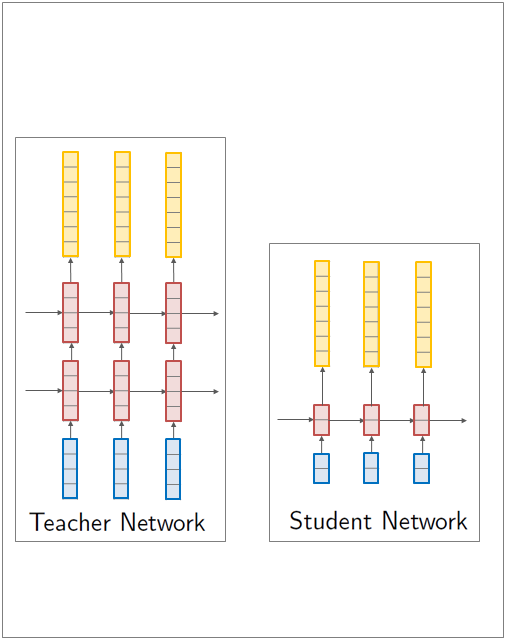
\includegraphics[width=5.5cm]{word-kd-1}
% \end{column}
% \end{columns}
% \end{frame}

\begin{frame}
\centerline{\structure{Baseline Model}}
\air 


\begin{columns}
\begin{column}{6.5cm}
Standard model minimize $\text{NLL}(\theta)$: 
\air
$$-\sum_t \log p(\wvec_t=y_t \given \wvec_{1:t-1}, \cvec ; \theta)$$

where $y_t$ is the ground truth word at time $t$.

\air 

Cross-entropy with ground truth.

\end{column}
\begin{column}{5.5cm}
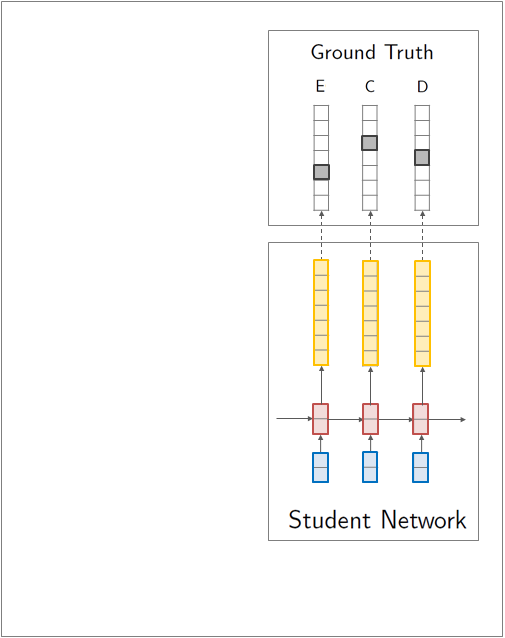
\includegraphics[width=5.5cm]{word-kd-0}
\end{column}
\end{columns}
\end{frame}

% \begin{frame}
% \centerline{\structure{Word-Level Knowledge Distillation}}
% \air
% \air
% \begin{columns}
% \begin{column}{6.5cm}
% Teacher network: $q(\wvec_{t} | \wvec_{1:t-1}, \cvec  ; \theta_T$)  \\
% \air
% \air
% Student network: $p(\wvec_{t} | \wvec_{1:t-1}, \cvec; \theta$)
% \end{column}
% \begin{column}{5.5cm}
% 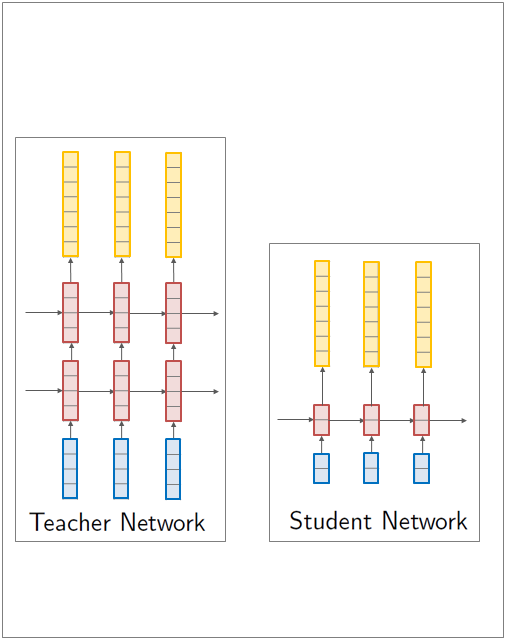
\includegraphics[width=5.5cm]{word-kd-1}
% \end{column}
% \end{columns}
% \end{frame}


\begin{frame}


\centerline{\structure{Word-Level Knowledge Distillation}}
\air 
\begin{columns}
\begin{column}{6.5cm}

Teacher network: $q(\wvec_{t} | \wvec_{1:t-1}, \cvec  ; \theta_T$)  
\air 

Minimize cross-entropy between teacher and student distribution  $\mathcal{L}_{\text{WORD-KD}}(\theta)$ \\

\begin{align*}
-\sum_t \sum_v &q(\wvec_t=v \given \wvec_{1: t-1}, \cvec ; \theta_T)\times \\
& \log p(\wvec_t =v \given \wvec_{1: t-1}, \cvec ; \theta)
\end{align*}
\end{column}

\begin{column}{5.5cm}
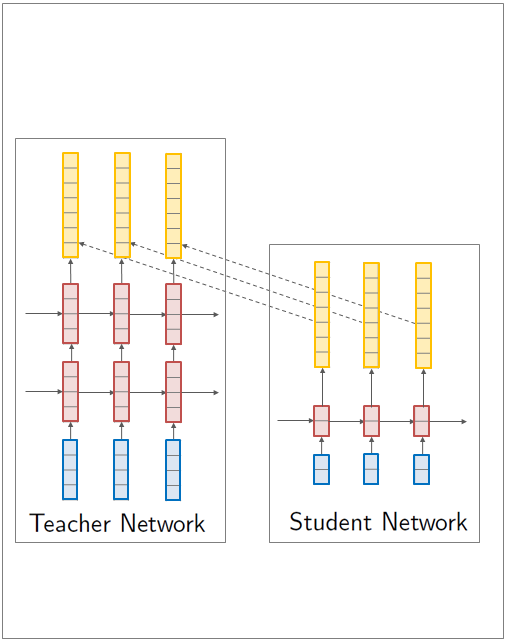
\includegraphics[width=5.5cm]{word-kd-2}
\end{column}
\end{columns}
\end{frame}

% \begin{frame}
% \centerline{\structure{Word-Level Knowledge Distillation}}
% \air
% \begin{columns}
% \begin{column}{6.5cm}
% Add a term for NLL (equivalent to minimizing cross-entropy between student a mixture distribution of teacher/data distributions)  
% \air
% $$\mathcal{L}(\theta) = \alpha\mathcal{L}_{\text{WORD-KD}}(\theta) + (1-\alpha)\mathcal{L}_{\text{NLL}}(\theta)$$
% \air
% $\alpha$ is a hyperparameter (we use $\alpha = 0.5$)
% \end{column}

% \begin{column}{5.5cm}
% 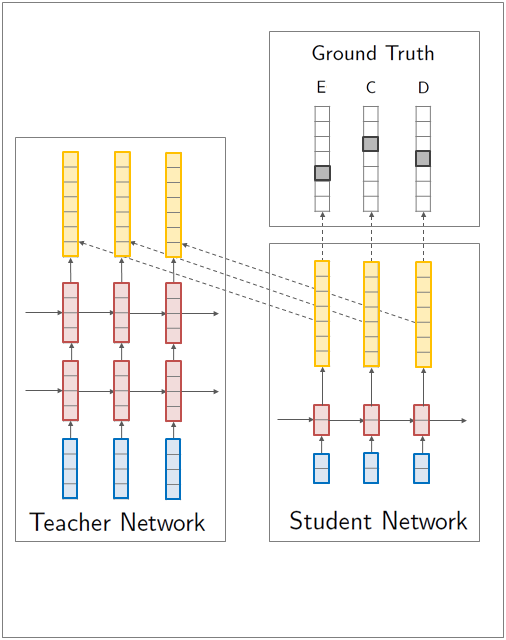
\includegraphics[width=5.5cm]{word-kd-3}
% \end{column}
% \end{columns}
% \end{frame}

\begin{frame}
\centerline{\structure{This Work: Sequence-Level Knowledge Distillation}}
\air 
\air
\air  

Instead of word NLL, 

\begin{align*}
-\sum_t \sum_v &q(\wvec_t=v \given \wvec_{1: t-1}, \cvec ; \theta_T)\times  \log p(\wvec_t =v \given \wvec_{1: t-1}, \cvec ; \theta)
\end{align*}
 
% $$-\sum_t \log p(\wvec_t=y_t \given \wvec_{1:t-1}, \cvec ; \theta)$$

Minimize cross-entropy between $q$ and $p$ implied \emph{sequence}-distributions 
\[
 -\sum_{\wvec_{1:T}} q(\wvec_{1:T} | \cvec; \theta_T) \times \log p(\wvec_{1:T} | \cvec ; \theta)
\]
\air

Note: Exponential sum over possible $\wvec_{1:T}$ . \\ 
\air
\air

\end{frame}

\begin{frame}
\centerline{\structure{A Simple Approximation}}
\air 
\air

%\centerline{Sequence-Level Knowledge Distillation}
\begin{columns}
\begin{column}{6cm}
Approximate $q(\wvec_{1:T} \given \cvec )$ with mode
$$q(\wvec_{1:T} \given \cvec ) \approx \mathbf{1}\{\argmax_{\wvec} q(\wvec_{1:T} \given \cvec )\}$$
\air
Roughly obtained wtih  beam search 
$$ \wvec^*_{1:T} \approx  \argmax_{\wvec_{1:T}} q(\wvec_{1:T} \given \cvec ) $$
\\
Empirically, point estimate captures 
significant mass

\end{column}
\begin{column}{6cm}
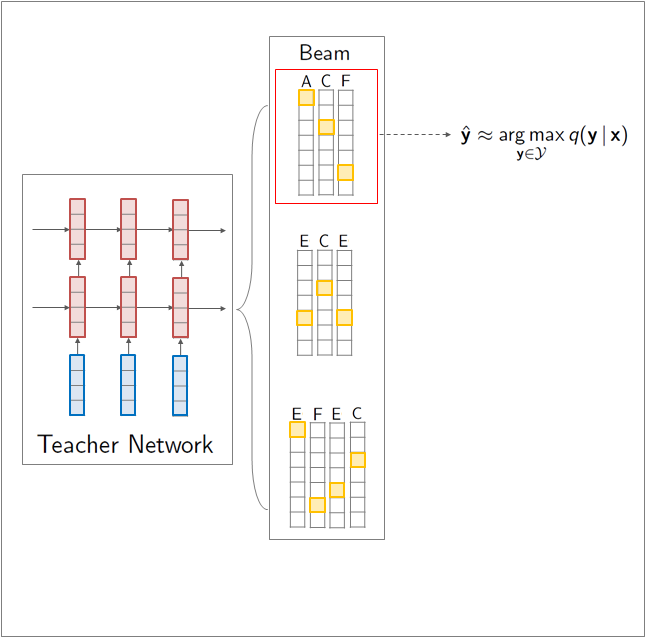
\includegraphics[width=6cm]{seq-kd-1}
\end{column}
\end{columns}
\end{frame}

\begin{frame}
\centerline{\structure{Sequence-Level Knowledge Distillation}}
\air
\air  
\begin{columns}
\begin{column}{5.5cm}
\begin{align*}

\mathcal{L}_\text{SEQ-KD}(\theta) &= -\log p(\wvec^*_{1:T} \given \cvec ; \theta)  \\
& \displaystyle \approx   -\sum_{\wvec_{1:T}} q(\wvec_{1:T} | \cvec; \theta_T) \log p(\wvec_{1:T} | \cvec ; \theta)
\end{align*}
Simplest model: train the student model on $\wvec^*$ with NLL
\end{column}
\begin{column}{5.5cm}
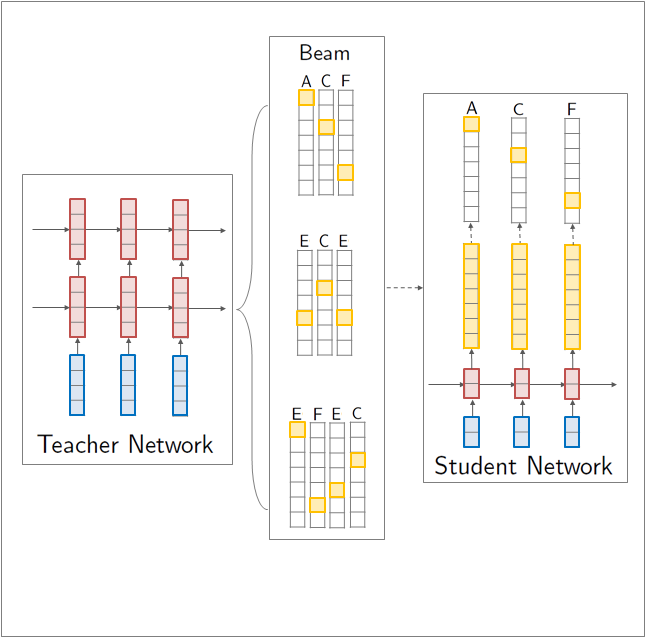
\includegraphics[width=5.5cm]{seq-kd-2}
\end{column}
\end{columns}
\end{frame}

\begin{frame}
\centerline{\structure{Results: English $\rightarrow$ German}}
\air
\air
\begin{table}
\centering
\small
\begin{tabular}{lccccrr}
\toprule
Model &    BLEU$_{K=1}$   & $\Delta_{K=1}$ & BLEU$_{K=5}$ & $\Delta_{K=5}$ & PPL & $p(\wvec^*)$ \\
\midrule
$4 \times 1000$ \\
Teacher    & $17.7$ &  $-$ & $19.5$&   $-$ &   $6.7$ &  $1.3\%$ \\
\hspace{1mm} Seq-Inter    & $19.6$ & $+1.9$&  $19.8$& $+0.3$&   $10.4$ & $8.2\%$   \\
\midrule
$2 \times 500$ \\ 
Student  $\,$   & $14.7$ & $-$ & $17.6$&  $-$ &  $8.2$ & $0.9\%$  \\
\hspace{1mm} Word-KD  & $15.4$ & $+0.7$& $17.7$& $+0.1$&  $8.0$ & $1.0\%$  \\
\hspace{1mm} Seq-KD   & $18.9$ & $+\mathbf{4.2}$& $19.0$& $+1.4$&  $22.7$ & $16.9\%$ \\
\hspace{1mm} Seq-Inter  & $18.9$ & $+\mathbf{4.2}$&$19.3$ & $+\mathbf{1.7}$ &  $15.8$ & $7.6\%$  \\
\bottomrule
\end{tabular}

\end{table}
\air
\air
\end{frame}

\begin{frame}
\centerline{\structure{Combining Knowledge Distillation and Pruning}}
\air
\air
\begin{table}[t] \label{prune}
\centering
\small
\begin{tabular}{l  r  r c  r }
\toprule
Model & Prune $\%$ & Params & BLEU & Ratio \\
\midrule 
$4 \times 1000$ & $0\%$ &$221$ m& $19.5$& $1 \times$   \\
$2 \times 500$ &  $0\%$& $84$ m& $19.3$& $3 \times$   \\
$2 \times 500$ & $50\%$& $42$ m&  $19.3$ & $5 \times$ \\
$2 \times 500$ &  $80\%$& $17$ m&  $19.1$ & $13 \times$ \\
$2 \times 500$ &  $85\%$& $13$ m&  $18.8$ & $18 \times$ \\
$2 \times 500$ &  $90\%$& $8$ m &  $18.5$  & $26 \times$ \\

\bottomrule
\end{tabular}
\end{table}
\end{frame}


\begin{frame}
  % \centerline{An Application}
  
  \begin{center}
    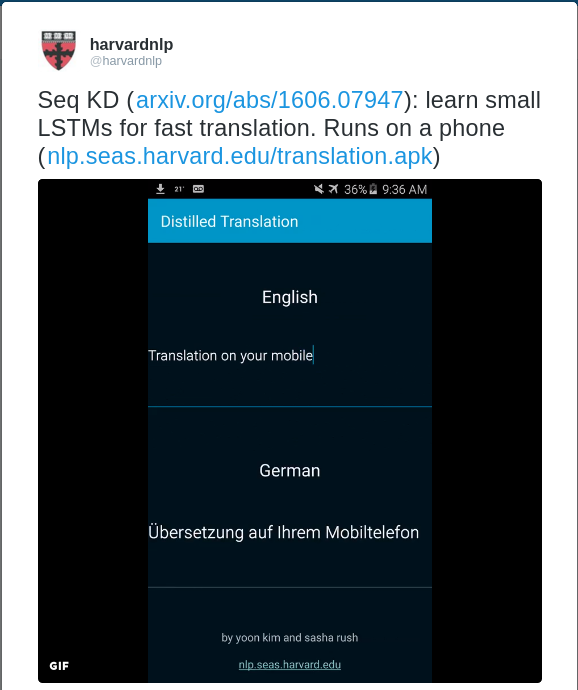
\includegraphics[height=0.9\textheight]{phonemt}
  \end{center}
\end{frame}

% \begin{frame}{Sequence-Level Interpolation}
% Sequence-level mixture of the teacher distribution and the data 
% \begin{align*}
%  \mathcal{L} (\theta) = -&\alpha\sum_{\yvec \in \mcY} q(\yvec \given \xvec; \theta_T) p(\yvec \given \xvec ; \theta)  \\
% & + (1-\alpha) p(\yvec = \wvec \given \xvec)
% \end{align*}
% Possible to approximate term with beam search and train on output from beam ($\hat{\yvec}$) and the ground truth ($\wvec$)---doubles the size of the training set.\\
% \air
% Consider a \emph{single-sequence} approximation to the mixture distribution.
% \end{frame}

% \begin{frame}{Sequence-Level Interpolation}
% \begin{columns}
% \begin{column}{6cm}
% Take the sequence that is on the beam but highest similarity function $sim$ (e.g. BLEU) to ground truth
% $$\tilde{\yvec} = \argmax_{\yvec_k \in \mathcal{T}_K} sim(\yvec_k, \wvec)$$
% where $\mathcal{T}_K$ is the $K$-best list from beam search.
% \end{column}
% \begin{column}{6cm}
% 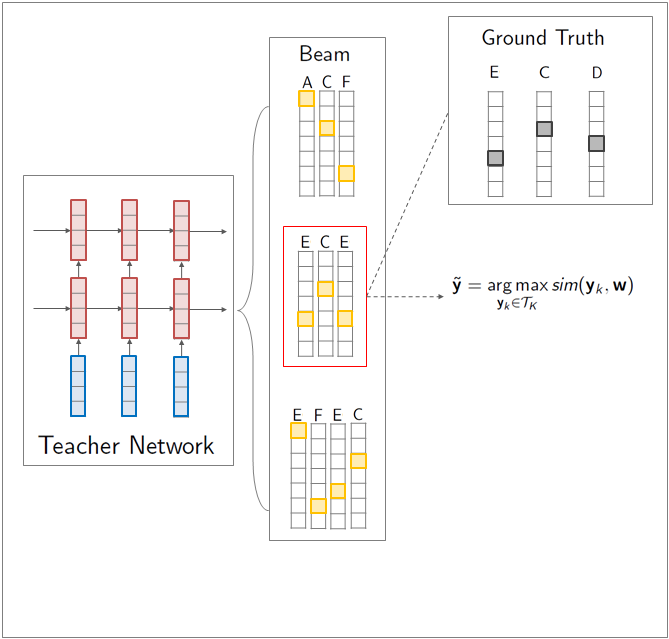
\includegraphics[width=6cm]{seq-inter-0}
% \end{column}
% \end{columns}
% \end{frame}

% \begin{frame}{Sequence-Level Interpolation}
% \begin{columns}
% \begin{column}{6cm}
% Train the student model on $\tilde{\yvec}$ with NLL.
% \end{column}
% \begin{column}{6cm}
% 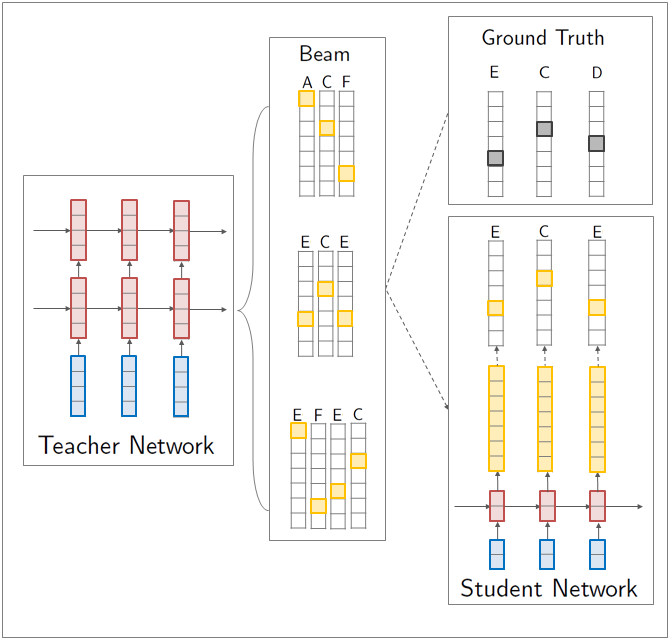
\includegraphics[width=6cm]{seq-inter-1}
% \end{column}
% \end{columns}
% \end{frame}

% % \begin{frame}{Convolutional Neural Networks (CNN)}{\Cite{LeCun1989}}
% % %   \textbf{Main Idea:} No morphology, use characters directly.
  
% % %   \begin{itemize}
% % %   \item Central network architecture  of deep learning in vision. 

% % % % in documenet

% %   \begin{center}
% %     \includegraphics[width=\textwidth]{../IACS/cnn_vision}
% %   \end{center}
% %   % \item Used for NLP tasks, often over the words. \Cite{Collobert2011,Kalchbrenner2014,Kim2014}
% %   % \end{itemize}  
% % \end{frame}

% % \begin{frame}{Convolutional Networks \Cite{DBLP:conf/eccv/ZeilerF14}}
% %   \includegraphics[height=0.9\textheight,trim={0 15cm 0 0},clip]{filters}
% % \end{frame}





% % \subsection{Deep Learning for Language}

% % \begin{frame}{Smoothness Image/Language}
% %   \only<1>{
% %   \begin{center}
% %     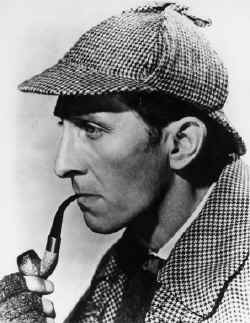
\includegraphics[width=3cm]{../IACS/holmes}
% %   \end{center}
% % }
% % \only<2>{
% %   \begin{center}
% %     \begin{tikzpicture}[spy using outlines={circle, magnification=30,
% %         size=3cm, connect spies}]
% %       \node {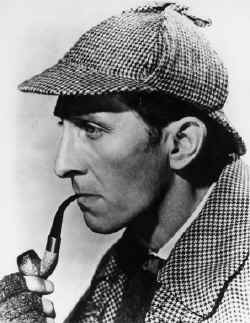
\includegraphics[width=3cm]{../IACS/holmes}}; 
% %       \spy [cyan] on
% %       (0.0,0.3) in node [left] at (5.4,-1.15);
% %     \end{tikzpicture}
% %   \end{center}
% % }
% %   \begin{quote}
% %     It is a capital mistake to theorize before one has
% %     \_\_\_\_. Insensibly one begins to twist facts to suit theories,
% %     instead of theories to suit facts. -Sherlock Holmes, A Scandal in Bohemia
% %   \end{quote}
% % \end{frame}

% % % \begin{frame}{Repair Image / Language \Cite{chatterjee2009application}}

% % %   \begin{center}
% % %     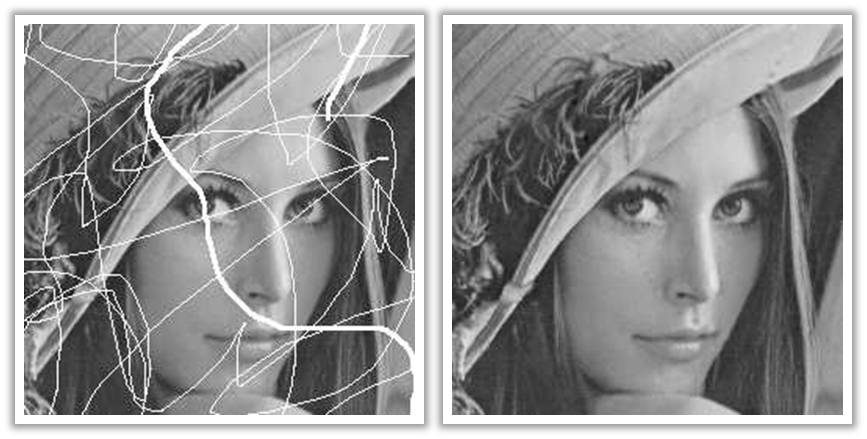
\includegraphics[width=6cm]{../IACS/lena}
% % %   \end{center}

% % %   \air
% % %   \only<1> {
% % %     \begin{quote}
% % %     It is a capital mistake to theorize before one has \_\_\_\_\_\_ $\ldots$ 
% % %     \end{quote}
% % %   }
% % %   \only<2> {
% % %     \begin{quote}
% % %       108 938 285 28 184 29 593 219 58 772 \_\_\_\_\_\_ $\ldots$ 
% % %     \end{quote}    
% % %   }
% % % \end{frame}

% % \begin{frame}
% %   \vspace{-1cm}
  
% %   \begin{center}
% %     \hspace*{-1cm}
% %     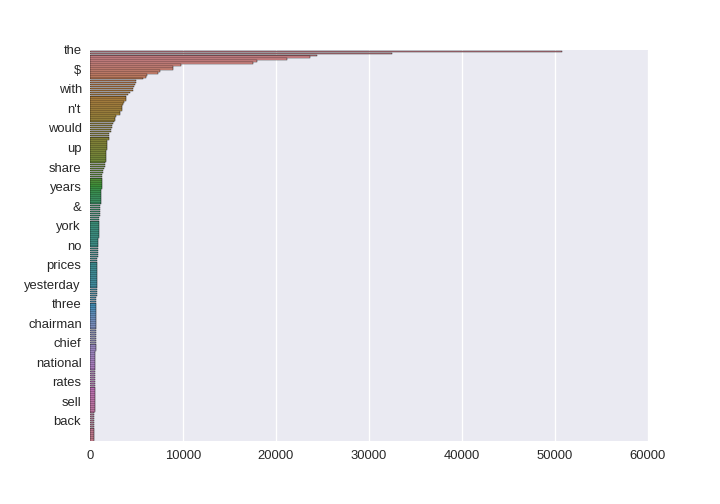
\includegraphics[width=1.2\textwidth]{zipf}
% %   \end{center}
% % \end{frame}


% % \begin{frame}{Word Embeddings}
% % \center
% % \includegraphics[width=12cm]{../../papers/lstm-char-cnn/slides/rnnlm1}
% % \end{frame}

% % \begin{frame}{Word Embeddings}
% % \center
% % \includegraphics[width=12cm]{../../papers/lstm-char-cnn/slides/rnnlm2}
% % \end{frame}


% % \begin{frame}
% %   \vspace{-5cm}
  
% %   \hspace*{-2cm}
% %   \includegraphics[width=1.5\textwidth]{graph}
% % \end{frame}


% % \begin{frame}{Recurrent Neural Network Model}
% % \center
% % \includegraphics[width=12cm]{../../papers/lstm-char-cnn/slides/rnnlm1}
% % \end{frame}
% % \begin{frame}{Recurrent Neural Network Model}
% % \center
% % \includegraphics[width=12cm]{../../papers/lstm-char-cnn/slides/rnnlm2}
% % \end{frame}
% % \begin{frame}{Recurrent Neural Network Model}
% % \center
% % \includegraphics[width=12cm]{../../papers/lstm-char-cnn/slides/rnnlm3}
% % \end{frame}
% % \begin{frame}{Recurrent Neural Network Model}
% % \center
% % 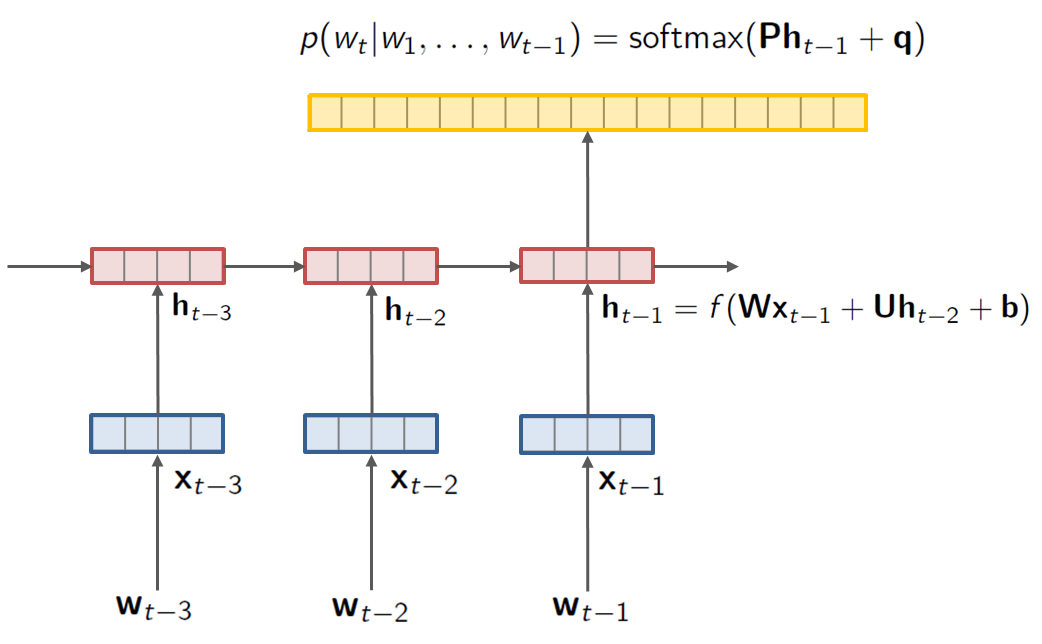
\includegraphics[width=12cm]{../../papers/lstm-char-cnn/slides/rnnlm4}
% % \end{frame}


% % \begin{frame}{Deep Learning Tools for NLP}
% %   \begin{itemize}
% %   \item \structure{Embeddings} convert discrete elements to dense representations.
% %     \air 

% %   \item \structure{Convolutions} learn filters for local structure 
% %     \air 
% %   \item \structure{RNNs} capture information in the ordering.

% %   \end{itemize}
% % \end{frame}

% \begin{frame}
%   \begin{center}
%     \structure{The Fantasy}
%   \end{center}
%   \begin{block}{}
%     \begin{quote}
%       I get pitched regularly by startups doing ‘generic machine
%       learning’ which is, in all honesty, a pretty ridiculous idea.
%       Machine learning is not undifferentiated heavy lifting, it’s not
%       commoditizable like EC2, and closer to design than coding.
%     \end{quote}
%   \end{block}
%   \begin{flushright}
%     - Joseph Reisinger (Computational Linguistics and Deep Learning)
%   \end{flushright}
% \end{frame}

% \begin{frame}% {Our Motivation: Trimming the Language Pipeline }
  
%   % \includegraphics[width=10cm]{arabic}
%   \begin{columns}
    
%     \begin{column}{0.6\linewidth}
%       \begin{center}
%         \includegraphics[width=6cm]{../IACS/arabic4}
%       \end{center}
%       \begin{center}
%         \includegraphics[width=5cm]{../IACS/arabic3}

%         \small{\Cite{marton2010improving}}
%       \end{center}

%     \end{column}
    
%     \begin{column}{0.4\linewidth}
%       {\small 
%         \alert{Pipeline Steps}
%       \begin{itemize}
%       \item Morphological Seg
%       \item Morphological Tagging
%       \item Part-of-Speech
%       \item Entity Recognition
%       \item Syntactic Parsing
%       \item Role Labeling
%       \item Discourse Analysis
%       \end{itemize}}
%     \end{column}

%   \end{columns}  
% \end{frame}


% % \begin{frame}{End-to-End Natural Language }
% %   \begin{itemize}
% %   \item Success in word-representantion and  
% %   \end{itemize}
% % \end{frame}


% \begin{frame}
%   \begin{center}
%     \structure{A Compromise?}
%   \end{center}

%   \begin{block}{}
%     \begin{quote}
%       Our field is the domain science of language technology; it's not
%       about the best method of machine learning - the central issue
%       remains the domain problems...  More of the field's effort
%       should go into problems, approaches, and architectures.
%     \end{quote}
%   \end{block}
%   \begin{flushright}
%     -Chris Manning (Computational Linguistics and Deep Learning)
%   \end{flushright}
% \end{frame}

% \begin{frame}
%   \begin{center}
%     This Talk
    
%     \alert{Language Structure of Two Domains }
%   \end{center}
%   \air 

%   \begin{itemize}
%   \item   \structure{Character-Aware Neural Models of Language (Yoon Kim)}
%     \air 

%   \begin{center}
%     \hspace*{-2cm}\includegraphics[scale=0.13]{../IACS/cnn8}
%   \end{center}


%   \item   Entity-Aware Neural Models for Coreference (Sam Wiseman)
%   \end{itemize}

%   \begin{center}
%     \includegraphics[scale=0.25]{justinexample}
%   \end{center}

%   \air 


% \end{frame}

% % \begin{frame}%{Our Motivation: Structure from Data}
% %   \begin{itemize}
% %   \item Can this explicit structure can be learned latently from data?
% %     \air 

% %   \item What architectural elements support our learning linguistic representations?
% %   \end{itemize}
%   % Projects:
  
%   % \begin{itemize}
%   % \item Character-Aware Language Models [CharCNN] 
%   % \item Coreference Resolution [Feature Embeddings] 
%   % \item Sentence Summarization [Contextual Attention] 
%   % \end{itemize}

% % \end{frame}

% \section{Character-Aware Language Models}


% \begin{frame}
%   \begin{block}{}
%     \begin{quote}
%       Although current deep learning research tends to claim to
%       encompass NLP, I'm (1) much less convinced about the strength of
%       the results, compared to the results in, say, vision ...
%     \end{quote}
%   \end{block}
%   \begin{flushright}
%     - Michael Jordan (2014) (Computational Linguistics and Deep Learning)
%   \end{flushright}

% \end{frame}

% % \begin{frame}
% % \center
% % \structure{RNN/LSTM Language Model}
% % \air 

% % \includegraphics[width=10cm]{../../papers/lstm-char-cnn/slides/rnnlm1}
% % \end{frame}
% % \begin{frame}
% % \center
% % \structure{RNN/LSTM Language Model}
% % \air 

% % \includegraphics[width=10cm]{../../papers/lstm-char-cnn/slides/rnnlm2}
% % \end{frame}
% % \begin{frame}
% % \center
% % \structure{RNN/LSTM Language Model}
% % \air 

% % \includegraphics[width=10cm]{../../papers/lstm-char-cnn/slides/rnnlm3}
% % \end{frame}
% \begin{frame}
% \center
% \structure{RNN/LSTM Language Model}
% \air 

% \includegraphics[width=10cm]{../../papers/lstm-char-cnn/slides/rnnlm4}
% \end{frame}

% \begin{frame}
%   \begin{center}
%     \structure{A Convincing Case?}
    
%     PTB Language Modeling
%   \end{center}
% \begin{table}
% \center
% \begin{tabular}{lcc}
%   \toprule
%  & Perplexity & Param Size \\ 
% \midrule
% KN-$5$ (as in Mikolov et al. 2012) & $141.2$ & $2$ \textsc{m}\\
% RNN (Mikolov et al. 2012)& $124.7$ & $6$ \textsc{m} \\
% LSTM-Medium (Zaremba et al. 2014) & $82.7$ & $20$ \textsc{m}\\
% LSTM-Huge (Zaremba et al. 2014) & $78.4$ & $52$ \textsc{m} \\
% \bottomrule
% \end{tabular}
% \end{table}
% \end{frame}


% % \begin{frame}
% %   \
% % \end{frame}



% % \begin{frame}{Language Modeling}
% %   % Learn distribution from data:
% %   % \[p(w_{t+1} | w_1, \ldots, w_{t})\]
% %   \begin{columns}    
% %     \begin{column}{0.5\textwidth}
% %   \begin{itemize}
% %   \item Speech Recognition
% %   \item Machine Translation
% %   \item Summarization
% %   \item Dialogue
% %   \item Soft Keyboards
% %   \item Word Correction
% %   \item Text Simplification
% %   \item $\ldots$
% %   \end{itemize}
% %   \end{column}


% %     \begin{column}{0.5\textwidth}
% %       \vspace{2cm}
     
% %       \includegraphics[width=5cm]{../IACS/siri}
% %     \end{column}
% %   \end{columns}

% % \end{frame}


% \begin{frame}
%   \begin{center}
%     \structure{Character-Aware Language Models}
%   \end{center}
% \end{frame}

% \begin{frame}
% \textbf{Challenge}: The fundamental unit of information is still the word.

% \air
 
% {\center
% \includegraphics[width=8cm]{emb} \\
% }
% \end{frame}

% \begin{frame}
% % \textbf{Issue}: The fundamental unit of information is still the \alert{word} 
%   \begin{center}
%     \structure{Our Friend Zipf}
%   \end{center}
% {\center
% \includegraphics[width=8cm]{../../papers/lstm-char-cnn/slides/zipf} \\
% }
% \end{frame}

% \begin{frame}
% % \textbf{Issue}: The fundamental unit of information is still the \alert{word} 
%   \begin{center}
%     \structure{Our Friend Zipf}
%   \end{center}

% {\center
% \includegraphics[width=8cm]{../../papers/lstm-char-cnn/slides/zipf2} \\
% }
% \air
% % Separate embeddings for ``trading'', ``trade'', ``trades", etc. \\
% \end{frame}

% % \begin{frame}{Character-Aware Language Models}
% %    \textbf{Issue:} Embeddings  different for: ``called'', ``call'', ``calling'', ``recalling'' and ``recalled''.
  
% %   \textbf{Goal}: Extend recurrent language model to exploit character structure.
% %   \begin{itemize}
% %     \item Share properties for ``close'' words. 
% %       \begin{center}
% %         \includegraphics[width=5cm]{../IACS/zipf}
% %       \end{center}
% %     \item Capture syntactic aspects of morphologically-rich languages.
% %   \end{itemize}
% % \end{frame}

% \begin{frame}%{Past Work}
%   \begin{center}
%     \structure{Past Work}

%     Explicit Morphological Segmentation
%   \end{center}
%   \begin{center}
%     recalling $\rightarrow$ re - call - ing

%   \end{center}\begin{itemize}
%     \item \cite{alexandrescu2006factored, bilmes2003factored}: Factored Language models with morphology.
%       \air 

%     \item  \cite{Luong2013}: LM with Recursive NN over morpheme embeddings 
%       \air


%     \item \cite{Botha2014}: LBL with sum over word/morpheme embeddings.
%   \end{itemize}
% \end{frame}

% % \begin{frame}{Convolutional Neural Networks (CNN)}{\Cite{LeCun1989}}
% %   \textbf{Main Idea:} No morphology, use characters directly.
  
% %   \begin{itemize}
% %   \item Central network architecture  of deep learning in vision. 

% % % in documenet

% %   \begin{center}
% %     \includegraphics[width=7cm]{IACS/cnn_vision}
% %     % \includemovie{1cm}{1cm}{lecun.gif}
% %   \end{center}
% %   \item Used for NLP tasks, often over the words. \Cite{Collobert2011,Kalchbrenner2014,Kim2014}
% %   \end{itemize}  
% % \end{frame}

% \begin{frame}

%   \begin{center}
%     \structure{Our Proposed Model}    
%   \end{center}

%   \begin{center}
%     \begin{tabular}{cclll}
%       1 & \structure{Embedding} &  sparse chars &$\Rightarrow$& dense features \\\\
%       2 & \structure{Convolution} &  char feature n-grams & $\Rightarrow$& dense word features  \\\\
%       3 & \structure{Pooling + NN} & variable length features & $\Rightarrow$& fixed length features \\\\
%       4 & \structure{LSTM} &  seq of word features  & $\Rightarrow$ & dense seq. features \\
%     \end{tabular}
%   \end{center}
% \end{frame}



% \begin{frame}%{Convolution into Recurrent Model}
%   \begin{center}
%     \includegraphics[width=9cm]{../IACS/lstm}
%   \end{center}
% \end{frame}

% \begin{frame}%{Convolution into Recurrent Model}
%     \begin{tabular}{cclll}
%       1 & \structure{Char Embedding} &  sparse chars &$\Rightarrow$& dense features \\\\
%       2 & \structure{CharCNN} &  char feature n-grams & $\Rightarrow$& dense word features  \\\\
%     \end{tabular}

%   \begin{center}
%     \includegraphics[width=9cm]{cnn}
%   \end{center}
% \end{frame}



% \begin{frame}%{Character Convolution (CharCNN)}
%   % \only<2> {
%   %   \[ \mathbf{Q} \in \mathbb{R}^{|\mathcal{C}| \times D} : \mbox{Matrix of character embeddings } \]
%   % }
%   % \only<3> {
%   %   \[ \mathbf{H} \in \mathbb{R}^{D \times w} : \mbox{Convolutional filter matrix of width } w=3 \]
%   % }

%   % \only<4>{\[\mathbf{h}[1] = \mbox{tanh}(\mathbf{C}[\ast, 1:3] \otimes \mathbf{H} + b)\]}

%   % \only<5>{\[\mathbf{h}[1] = \mbox{tanh}(\mathbf{C}[\ast, 1:3] \otimes \mathbf{H} + b)\]}

%   % \only<6>{\[\mathbf{h}[2] = \mbox{tanh}(\mathbf{C}[\ast, 2:4] \otimes \mathbf{H} + b)\]}

%   % \only<7>{\[\mathbf{h}[T-2] = \mbox{tanh}(\mathbf{C}[\ast, T-2:T] \otimes \mathbf{H} + b)\]}

%   % \only<8>{\[y[1] = \max_{i} \mathbf{h}[i]\]}


%   % \only<9>{\[\mathbf{h'}[1] = \mbox{tanh}(\mathbf{C}[\ast, 1:2] \otimes \mathbf{H'} + b')\]}

%   % \only<10>{\[y[2] = \max_{i} \mathbf{h'}[i]\]}


%   \begin{center}
%     \foreach \y in {1,2,3,4,5,6,7,8,9,10} {
%       \includegraphics<\y>[width=0.8\linewidth]{../IACS/cnn\y} }
%   \end{center}
% \end{frame}


% \begin{frame}%{Highway Network}
% % \vspace{-2mm}
% % \center
%   \begin{center}
%     \includegraphics[width=7.6cm]{../../papers/lstm-char-cnn/slides/hw}
%   \end{center}
% \end{frame}

% \begin{frame}
% \center
%   \begin{center}
%     \begin{tabular}{cclll}
%       \structure{Highway Network} & & dense features &$\Rightarrow$& dense features \\\\
%       \end{tabular}

%       ``gated multi-layer perceptron''
%     \end{center}

%     \air 
%     \air 

% \includegraphics[width=10cm]{../../papers/lstm-char-cnn/slides/hw2_annotated}
% \end{frame}


% \begin{frame}
%   \begin{center}
%     \structure{Results}
%   \end{center}
% \end{frame}

% % \begin{frame}{Convolution into Recurrent Model}
% %   \begin{center}
% %     \includegraphics[width=7cm]{../IACS/lstm}
% %   \end{center}
% % \end{frame}

% \begin{frame}%{Results: English PTB}
% \begin{table}
% \center
% \begin{tabular}{lcc}
% \toprule
%  & Perplexity & Param Size \\ 
% \midrule
% LSTM-Word-Small & $97.6$ & $5$ \textsc{m}\\
% \textbf{LSTM-CharCNN-Small} & $92.3$ & $5$ \textsc{m}\\
% LSTM-Word-Large & $85.4$ & $20$ \textsc{m}\\
% \textbf{LSTM-CharCNN-Large} & $78.9$ & $19$ \textsc{m}\\ 
% \midrule
% KN-$5$ (Mikolov et al. 2012) & $141.2$ & $2$ \textsc{m}\\
% RNN (Mikolov et al. 2012)& $124.7$ & $6$ \textsc{m} \\
% LSTM-Medium (Zaremba et al. 2014) & $82.7$ & $20$ \textsc{m}\\
% LSTM-Huge (Zaremba et al. 2014) & $78.4$ & $52$ \textsc{m} \\
% \bottomrule
% \end{tabular}
% \end{table}
% \end{frame}


% % \begin{frame}%{Data}
% % \begin{table}
% % \center
% % \begin{tabular}{lcccccc}
% % \toprule
% % & \multicolumn{3}{c}{\textsc{Data-s}} & \multicolumn{3}{c}{\textsc{Data-l}} \\
% %  & $|\mathcal{V}|$ & $|\mathcal{C}|$ & $T$  & $|\mathcal{V}|$ & $|\mathcal{C}|$ & $T$ \\
% % \midrule
% % English (\textsc{En}) & $10$ \textsc{k} & $51$ & $1$ \textsc{m} & $60$ \textsc{k} & $129$ & $20$ \textsc{m}  \\ 
% % Czech (\textsc{Cs}) & $46$ \textsc{k} &  $93$ & $1$ \textsc{m}  & $206$ \textsc{k} & $127$ & $17$ \textsc{m}  \\ 
% % German (\textsc{De})  & $36$ \textsc{k} &  $75$ & $1$ \textsc{m}  & $339$ \textsc{k} & $140$ & $51$ \textsc{m}  \\ 
% % Spanish (\textsc{Es}) & $27$ \textsc{k} &  $72$ & $1$ \textsc{m}  & $152$ \textsc{k} & $130$ & $56$ \textsc{m}  \\ 
% % French (\textsc{Fr}) & $25$ \textsc{k} &  $77$ & $1$ \textsc{m}   & $137$ \textsc{k} & $133$ & $57$ \textsc{m}  \\ 
% % Russian (\textsc{Ru})  & $62$ \textsc{k} &  $64$ & $1$ \textsc{m}   & $497$ \textsc{k} & $114$ & $25$ \textsc{m} \\
% % \bottomrule
% % \end{tabular}
% % \end{table}
% % \air
% % \air
% % Small English data is the English Penn Treebank (PTB). Rest comes from the 2013 ACL Workshop on Machine Translation. \\
% % \end{frame}

% \begin{frame}%{Data}
% \begin{table}
% \center
% \begin{tabular}{lrrcrrc}
% & \multicolumn{3}{c}{\textsc{Data-s}} & \multicolumn{3}{c}{\textsc{Data-l}} \\
%  & $|\mathcal{V}|$ & $|\mathcal{C}|$ & $T$  & $|\mathcal{V}|$ & $|\mathcal{C}|$ & $T$ \\
% \cmidrule(lr){2-4}  \cmidrule(lr){5-7}
% English (\textsc{En}) & $10$ k & $51$ & $1$ m & $60$ k & $197$ & $20$ m  \\ 
% Czech (\textsc{Cs}) & $46$ k &  $101$ & $1$ m  & $206$ k & $195$ & $17$ m  \\ 
% German (\textsc{De})  & $37$ k &  $74$ & $1$ m  & $339$ k & $260$ & $51$ m  \\ 
% Spanish (\textsc{Es}) & $27$ k &  $72$ & $1$ m  & $152$ k & $222$ & $56$ m  \\ 
% French (\textsc{Fr}) & $25$ k &  $76$ & $1$ m   & $137$ k & $225$ & $57$ m  \\ 
% Russian (\textsc{Ru})  & $62$ k &  $62$ & $1$ m   & $497$ k & $111$ & $25$ m \\
% \end{tabular}
% \end{table}
% \air

% \begin{center}
%   $|\mcV| = $ Word vocab Size \\ $|\mathcal{C}| = $ Character vocab
%   size \\ $T = $ number of tokens in training set.
% \end{center}
% \end{frame}

% \begin{frame}
% \begin{table}
% \center
% \begin{tabular}{lrrcrrc}
% & \multicolumn{3}{c}{\textsc{Data-s}} & \multicolumn{3}{c}{\textsc{Data-l}} \\
%  &   $|\mathcal{V}|$ & $|\mathcal{C}|$ & $T$  & $|\mathcal{V}|$ & $|\mathcal{C}|$ & $T$ \\
% \cmidrule(lr){2-4}  \cmidrule(lr){5-7}
% English (\textsc{En}) &  $10$ k & $51$ & $1$ m &  {\color{red} $60$ k} & $197$ & {\color{red} $20$ m}  \\ 
% Czech (\textsc{Cs}) &     $46$ k &  $101$ & $1$ m  & $206$ k & $195$ & $17$ m  \\ 
% German (\textsc{De})  &     $37$ k &  $74$ & $1$ m  &  $339$ k & $260$ & $51$ m  \\ 
% Spanish (\textsc{Es}) &    $27$ k &  $72$ & $1$ m  & $152$ k & $222$ & $56$ m  \\ 
% French (\textsc{Fr}) &     $25$ k &  $76$ & $1$ m   &   $137$ k & $225$ & $57$ m  \\ 
% Russian (\textsc{Ru})   &   $62$ k &  $62$ & $1$ m   &  {\color{red} $497$ k} & $111$ &  {\color{red} $25$ m} \\
% \end{tabular}
% \end{table}
% % \air
% % \air
% % $|\mcV|$ varies quite a bit by language.\\ \air 
% % (effectively use the full vocabulary)
% \begin{center}
%   $|\mcV| = $ Word vocab Size \\ $|\mathcal{C}| = $ Character vocab
%   size \\ $T = $ number of tokens in training set.
% \end{center}

% \end{frame}

% \begin{frame}
%   \begin{center}
%     \structure{Baselines}
%   \end{center}

% \textbf{Kneser-Ney LM}: Count-based baseline \\
% \air 
% \air
% \textbf{Word LSTM}: Word embeddings as input \\
% \air
% \air 
% \textbf{Morpheme LBL} (\cite{Botha2014}) \\
% \air
% Input for word $k$ is
% $$
% \underbrace{\mathbf{x}^k}_\text{word embedding} + \underbrace{\sum_{j \in \mathcal{M}_k} \mathbf{m}^j}_\text{morpheme embeddings}
% $$	
% \air
% \textbf{Morpheme LSTM}: Same input as above, but with LSTM architecture

% % Morphemes obtained from running an unsupervised morphological tagger 
% % Morfessor Cat-MAP {\footnotesize (\cite{Creutz2007})}.
% \end{frame}


% % \begin{frame}{Perplexity on Data-S (1 M Tokens)}
% % \center
% % \includegraphics[width=12cm]{results1}
% % \end{frame}

% % \begin{frame}{Perplexity on Data-S (1 M Tokens)}
% % \center
% % \includegraphics[width=12cm]{results2}
% % \end{frame}

% % \begin{frame}{Perplexity on Data-S (1 M Tokens)}
% % \center
% % \includegraphics[width=12cm]{results3}
% % \end{frame}

% % \begin{frame}{Perplexity on Data-S (1 M Tokens)}
% % \center
% % \includegraphics[width=12cm]{results4}
% % \end{frame}

% % \begin{frame}{Perplexity on Data-S (1 M Tokens)}
% % \center
% % \includegraphics[width=12cm]{results5}
% % \end{frame}


% % \begin{frame}{Perplexity on Data-L (17-57 M Tokens)}
% % \center
% % \includegraphics[width=12cm]{results6}
% % \end{frame}


% \begin{frame}
%   \begin{center}
%     \structure{Perplexity on Data-S (1 M Tokens)}
%   \end{center}
%   \begin{center}
%     % \foreach \y in {1,2,3,4} {
%       \includegraphics[width=\linewidth]{../../papers/lstm-char-cnn/slides/results5}
%   \end{center}
% \end{frame}

% \begin{frame}
%   \begin{center}
%     \structure{Perplexity on Data-L (17-57 M Tokens)}
%   \end{center}
%   \begin{center}
%     \includegraphics[width=12cm]{../../papers/lstm-char-cnn/slides/results6}
%   \end{center}
% \end{frame}


% % \begin{frame}{Results: Large Datasets}
% % \begin{table}
% % \center
% % \begin{tabular}{llcccccc}
% % \toprule
% % && \textsc{Cs} & \textsc{De} & \textsc{Es} & \textsc{Fr} &  \textsc{Ru} & \textsc{En} \\
% % \midrule
% % \multirow{2}{*}{B\&B} & KN-$4$ & $862$ & $463$ & $219$ & $243$ & $390$ & $291$ \\
% % &  MLBL & $643$ & $404$ & $203$ & $227$ & $\mathbf{300}$ & $273$ \\
% % \midrule
% % \multirow{3}{*}{Small}&  Word & $701$ & $347$ & $186$ & $202$ & $353$ & $236$ \\
% % &  Morph & $615$ & $331$ & $189$ & $209$ & $331$ & $233$ \\
% % &  Char & $\mathbf{587}$ & $\mathbf{298}$ & $\mathbf{168}$ & $\mathbf{191}$ & $313$ & $\mathbf{214}$ \\
% % \bottomrule
% % \end{tabular}
% % \end{table}
% % % \air
% % % Only trained the small models on the large datasets due to memory constraints (2GB)\\
% % % \air
% % % Difference in size is greater for non-PTB because morpheme/word levels are more sensitive to $|\mathcal{V}|$
% % % (e.g. on small Russian dataset LSTM-CharCNN Large has 54M parameters whereas the large word model has
% % % 89M parameters).
% % \end{frame}


% \begin{frame}%{Learned Word Representations (In Vocab)}

% \vspace{-5mm}
% \begin{table}
% \center
% \small
% \begin{tabular}{cccccc}
% & \multicolumn{5}{c}{\textbf{In Vocabulary}}  \\
% & while & his & you & richard & trading \\
% \cmidrule(lr){2-6}
% & although & your & conservatives & jonathan & advertised \\
% { Word}		& letting & her & we & robert & advertising \\
% { Embedding}		& though & my & guys & neil & turnover \\
% 			& minute & their & i & nancy & turnover \\
% \addlinespace
% \addlinespace
% \pause
% 	& chile & this & your & hard & heading \\
% { \textbf{Characters}} 	& whole & hhs & young & rich& training \\
% { (before highway)}	& meanwhile & is & four & richer & reading \\
% 			& white & has & youth & richter & leading  \\
% \addlinespace
% \addlinespace
% \pause
% 			& meanwhile & hhs & we & eduard & trade \\
% { \textbf{Characters}}	& whole & this & your & gerard & training   \\
% { (after highway)}	& though & their & doug & edward & traded \\
% 			& nevertheless & your & i & carl & trader \\
% \end{tabular}
% \end{table}
% \end{frame}


% \begin{frame}%{Learned Word Representations (In Vocab)}

% \vspace{-5mm}
% \begin{table}
% \center
% \small
% \begin{tabular}{cccccc}
% & \multicolumn{5}{c}{\textbf{In Vocabulary}}  \\
% & while & his & you & richard & \color{red}{trading} \\
% \cmidrule(lr){2-6}
% & although & your & conservatives & jonathan & advertised \\
% { Word}		& letting & her & we & robert & advertising \\
% { Embedding}		& though & my & guys & neil & turnover \\
% 			& minute & their & i & nancy & turnover \\
% \addlinespace
% \addlinespace
% 	& chile & this & your & hard & \color{red}{heading} \\
% { \textbf{Characters}} 	& whole & hhs & young & rich& \color{red}{training} \\
% { (before highway)}	& meanwhile & is & four & richer & \color{red}{reading} \\
% 			& white & has & youth & richter & \color{red}{leading}  \\
% \addlinespace
% \addlinespace
% 			& meanwhile & hhs & we & eduard & trade \\
% { \textbf{Characters}}	& whole & this & your & gerard & training   \\
% { (after highway)}	& though & their & doug & edward & traded \\
% 			& nevertheless & your & i & carl & trader \\
% \end{tabular}
% \end{table}
% \end{frame}

% \begin{frame}%{Learned Word Representations (In Vocab)}

% \vspace{-5mm}
% \begin{table}
% \center
% \small
% \begin{tabular}{cccccc}
% & \multicolumn{5}{c}{\textbf{In Vocabulary}}  \\
% & \color{red}{while} & his & you & richard & trading \\
% \cmidrule(lr){2-6}
% & although & your & conservatives & jonathan & advertised \\
% { Word}		& letting & her & we & robert & advertising \\
% { Embedding}		& though & my & guys & neil & turnover \\
% 			& minute & their & i & nancy & turnover \\
% \addlinespace
% \addlinespace
% 	& \color{red}{chile} & this & your & hard & heading \\
% { \textbf{Characters}} 	& \color{red}{whole} & hhs & young & rich& training \\
% { (before highway)}	& meanwhile & is & four & richer & reading \\
% 			& \color{red}{white} & has & youth & richter & leading  \\
% \addlinespace
% \addlinespace
% 			& meanwhile & hhs & we & eduard & trade \\
% { \textbf{Characters}}	& whole & this & your & gerard & training   \\
% { (after highway)}	& though & their & doug & edward & traded \\
% 			& nevertheless & your & i & carl & trader \\
% \end{tabular}
% \end{table}
% \end{frame}

% \begin{frame}%{Learned Word Representations (In Vocab)}

% \vspace{-5mm}
% \begin{table}
% \center
% \small
% \begin{tabular}{cccccc}
% & \multicolumn{5}{c}{\textbf{In Vocabulary}}  \\
% & while & his & you & richard & \color{red}{trading} \\
% \cmidrule(lr){2-6}
% & although & your & conservatives & jonathan & advertised \\
% { Word}		& letting & her & we & robert & advertising \\
% { Embedding}		& though & my & guys & neil & turnover \\
% 			& minute & their & i & nancy & turnover \\
% \addlinespace
% \addlinespace
% 	& chile & this & your & hard & heading \\
% { \textbf{Characters}} 	& whole & hhs & young & rich& training \\
% { (before highway)}	& meanwhile & is & four & richer & reading \\
% 			& white & has & youth & richter & leading  \\
% \addlinespace
% \addlinespace
% 			& meanwhile & hhs & we & eduard & \color{red}{trade} \\
% { \textbf{Characters}}	& whole & this & your & gerard & \color{red}{training}   \\
% { (after highway)}	& though & their & doug & edward & \color{red}{traded} \\
% 			& nevertheless & your & i & carl & \color{red}{trader} \\
% \end{tabular}
% \end{table}
% \end{frame}

% \begin{frame}%{Learned Word Representations (In Vocab)}

% \vspace{-5mm}
% \begin{table}
% \center
% \small
% \begin{tabular}{cccccc}
% & \multicolumn{5}{c}{\textbf{In Vocabulary}}  \\
% & \color{red}{while} & his & you & richard & trading \\
% \cmidrule(lr){2-6}
% & although & your & conservatives & jonathan & advertised \\
% { Word}		& letting & her & we & robert & advertising \\
% { Embedding}		& though & my & guys & neil & turnover \\
% 			& minute & their & i & nancy & turnover \\
% \addlinespace
% \addlinespace
% 	& chile & this & your & hard & heading \\
% { \textbf{Characters}} 	& whole & hhs & young & rich& training \\
% { (before highway)}	& meanwhile & is & four & richer & reading \\
% 			& white & has & youth & richter & leading  \\
% \addlinespace
% \addlinespace
% 			& meanwhile & hhs & we & eduard & trade \\
% { \textbf{Characters}}	& whole & this & your & gerard & training   \\
% { (after highway)}	& \color{red}{though} & their & doug & edward & traded \\
% 			& \color{red}{nevertheless} & your & i & carl & trader \\
% \end{tabular}
% \end{table}
% \end{frame}

% \begin{frame}%{Learned Word Representations (OOV)}

% \begin{table}[!t]
% \center
% \small
% \begin{tabular}{cccc}
% & \multicolumn{3}{c}{{ \textbf{Out-of-Vocabulary}}} \\
% & computer-aided & misinformed & looooook \\
% \cmidrule(lr){2-4}
% 	& computer-guided & informed & look \\
% {\textbf{Characters}}	& computerized & performed  & cook\\
% { (before highway)}& disk-drive & transformed & looks\\
% 			& computer & inform & shook \\
% \addlinespace
% \addlinespace
% 			& computer-guided & informed & look\\
% { \textbf{Characters}}	 & computer-driven & performed & looks  \\
% { (after highway)}	 & computerized& outperformed & looked \\
% 			& computer & transformed & looking \\

% \end{tabular}
% \end{table}
% \end{frame}

% \begin{frame}%{Learned Word Representations (OOV)}

% \begin{table}[!t]
% \center
% \small
% \begin{tabular}{cccc}
% & \multicolumn{3}{c}{{ \textbf{Out-of-Vocabulary}}} \\
% & computer-aided & misinformed & \color{red}{looooook} \\
% \cmidrule(lr){2-4}
% 	& computer-guided & informed & \color{red}{look} \\
% {\textbf{Characters}}	& computerized & performed  & \color{red}{cook}\\
% { (before highway)}& disk-drive & transformed & \color{red}{looks}\\
% 			& computer & inform & \color{red}{shook} \\
% \addlinespace
% \addlinespace
% 			& computer-guided & informed & look\\
% { \textbf{Characters}}	 & computer-driven & performed & looks  \\
% { (after highway)}	 & computerized& outperformed & looked \\
% 			& computer & transformed & looking \\
% \end{tabular}
% \end{table}
% \end{frame}


% \begin{frame}%{Learned Word Representations (OOV)}

% \begin{table}[!t]
% \center
% \small
% \begin{tabular}{cccc}
% & \multicolumn{3}{c}{{ \textbf{Out-of-Vocabulary}}} \\
% & computer-aided & misinformed & \color{red}{looooook} \\
% \cmidrule(lr){2-4}
% 	& computer-guided & informed & look \\
% {\textbf{Characters}}	& computerized & performed  & cook\\
% { (before highway)}& disk-drive & transformed & looks\\
% 			& computer & inform & shook \\
% \addlinespace
% \addlinespace
% 			& computer-guided & informed & \color{red}{look}\\
% { \textbf{Characters}}	 & computer-driven & performed & \color{red}{looks}  \\
% { (after highway)}	 & computerized& outperformed & \color{red}{looked} \\
% 			& computer & transformed & \color{red}{looking} \\
% \end{tabular}
% \end{table}
% \end{frame}

% \begin{frame}%{Convolutional Layer}
% Does each filter truly pick out a character $n$-gram?

% \begin{center}
%   \includegraphics[width=6cm]{../../papers/lstm-char-cnn/slides/visualizing_filters}
% \end{center}
% \end{frame}

% \begin{frame}%{Convolutional Filters}
% For each filter, visualize 100 substrings with the highest filter response

% \begin{center}
%   \includegraphics[width=6cm]{../../papers/lstm-char-cnn/slides/ed_best.png}
% \end{center}
% \end{frame}

% \begin{frame}%{Convolutional Filters}
% For each filter, visualize 100 substrings with the highest filter response

% \begin{center}
%   \includegraphics[width=6cm]{../../papers/lstm-char-cnn/slides/ies_best.png}
% \end{center}
% \end{frame}


% % \begin{frame}{Applications}
  
% % \end{frame}

% \begin{frame}
%   \begin{center}
%     \structure{Applications of This Work}
%   \end{center}

%   \begin{itemize}
%   \item 1 billion token LM version from Google  \Cite{DBLP:journals/corr/JozefowiczVSSW16}
%     \air 

%   \item Improvements in machine translation  \Cite{2016arXiv160300810C}
%     \air
 
%   \item Grammatical error correction {\footnotesize (Schmaltz et al, 2016)}
%   \end{itemize}

%   Much other recent work on character inputs:
%   \begin{itemize}
%   \item \cite{Santos2014a}: CNN over characters concatenated with word embeddings into CRF.
%   \item \cite{Ballesteros2015}: LSTM over characters for parsing.
%   \item \cite{Ling2015}: LSTM over characters into another LSTM for language modeling/POS-tagging.
%   \end{itemize}

% \end{frame}


% \begin{frame}


%   \begin{center}
%     \alert{AESW16} \\
%     \structure{Task:} Grammatical Error Identification
%   \end{center}

%   \begin{itemize}
%   \item ~500K sentences containing annotated edits
%   \item Domain of academic and scientific writing
%   \item Task is to identify sentences with mistakes
%   \end{itemize}
%   \air 

%   \textbf{Example:}
%   \texttt{The proof of -LRB- ii -RRB- comes from the convex analysis of operators , <del> on </del> which we omit here -LRB- see CITE -RRB- .}

% \end{frame}


% \begin{frame}
%   \begin{center}
%     \includegraphics[width=11cm]{../../papers/AESW2016atBEA11/aesw/images/grammar}
%   \end{center}
% \end{frame}

% \begin{frame}

%   \begin{center}
%     \structure{Development Results}
%   \end{center}
% \begin{table}[ht!]
% \centering
% \footnotesize
% \begin{tabular}{lccc}
% \toprule
% Model & Precision & Recall & $F_1$ \\
% \midrule
% \textsc{Random} & $0.3885$ & $0.4992$ & $0.4369$ \\
% \midrule
% \textsc{CNN-static} &  $0.5349$ & $0.7586$ & $0.6274$ \\
% \textsc{CNN-nonstatic} &  $0.5365$ & $0.7758$ & $0.6343$ \\
% \midrule
% \textsc{Word+all} & $0.5399$ & $0.7882$ & $0.6408$ \\
% \textsc{Word+sample} &  $0.5394$ & $0.8024$ & $0.6451$ \\
% \textsc{Char+all} &  $0.5400$ & $0.8048$ & $0.6463$ \\
% \textsc{Char+sample} &  $0.5526$ & $0.8126$ & $0.6579$ \\
% \bottomrule
% \end{tabular}
% % \caption{Experimental results on the development set excluding the held-out 10k tuning subset.}
% \label{tab:dev-results}
% \end{table}
% \end{frame}

% \begin{frame}
%   \centering
%   \structure{AESW16}
%   \air 

%   \begin{tabular}{lcccc}
% \toprule
% Model & Precision & Recall & $F_1$ \\
% \midrule
% \textsc{Random} & $0.3607$ & $0.6004$ & $0.4507$ \\
% \midrule
% \textsc{Knowlet} &  $0.6241$ & $0.3685$ & $0.4634$ \\
% \textsc{NTNU-YZU} &  $0.6717$ & $0.3805$ & $0.4858$ \\
% \textsc{HITS} &  $0.3765$ & $0.948$ & $0.5389$ \\
% \textsc{UW-SU} & $0.4145$ & $0.8201$ & $0.5507$ \\
% \textsc{NTNU-YZU} &  $0.5025$ & $0.7785$ & $0.6108$ \\
% \midrule
% \textsc{Char+sample} &  $0.5112$ & $0.7841$ & $0.6189$ \\
% \textsc{Combination} &  $0.5444$ & $0.7413$ & $0.6278$ \\
% \bottomrule
% \end{tabular}

% \end{frame}

% \begin{frame}
%   \begin{center}
%     This Talk
    
%     \alert{Language Structure of Two Domains }
%   \end{center}
%   \air 

%   \begin{itemize}
%   \item   Character-Aware Neural Models of Language (Yoon Kim)
%     \air 

%   \begin{center}
%     \hspace*{-2cm}\includegraphics[scale=0.13]{../IACS/cnn8}
%   \end{center}

%   \item   \structure{Entity-Aware Neural Models for Coreference (Sam Wiseman)}
%   \end{itemize}

%   \begin{center}
%     \includegraphics[scale=0.25]{justinexample}
%   \end{center}

%   \air 
% \end{frame}


% \section{Coreference Resolution}

% % \begin{frame}
% %   \textbf{Coreference Resolution {\small \citep{wiseman15learning}}}
% % \end{frame}

% % \begin{frame}{Information Extraction}
% %   \begin{center}
% %     \includegraphics[width=\textwidth]{cort}
% %   \end{center}
% % \end{frame}

% \begin{frame}
% % \frametitle{Coreference Resolution}
% \begin{quote}
% {\Large
% Cadillac posted a 3.2\% increase despite new competition from Lexus, the fledgling luxury-car division of Toyota Motor Corp.
% Lexus sales weren't available; the cars are imported and Toyota reports their sales only at month-end.}
% \end{quote}
% \end{frame}


% \begin{frame}
% % \frametitle{Coreference Resolution}
% \begin{tikzpicture}
% \node (q) at (current page.center) {
% \begin{quote}
% {\Large \lbbrack Cadillac\rbbrack posted a \lbbrack 3.2\% increase\rbbrack despite \lbbrack new competition from \textcolor{vermillion}{\lnbrack Lexus, the fledgling luxury-car division of \textcolor{myblue}{\lnbrack Toyota Motor Corp\rnbrack}\rnbrack}\rbbrack.
% \lbbrack\textcolor{vermillion}{\lnbrack Lexus\rnbrack} sales\rbbrack weren't available; \lbbrack the cars\rbbrack are imported and \textcolor{myblue}{\lnbrack Toyota\rnbrack} reports \lbbrack\textcolor{myblue}{\lnbrack their\rnbrack} sales\rbbrack only at \lbbrack month-end\rbbrack.}
% \end{quote}
% };
% \end{tikzpicture}
% \end{frame}


% \begin{frame}
% %\frametitle{Mention Ranking}{\Cite{DandB:08,BandR:08}}

% % \begin{itemize}
% % \item Model each mention $x$ as having a single ``true'' antecedent
% % \item Score potential antecedents $y$ of each mention $x$ with a scoring function $s(x,y)$
% % \item $\mcY(x) = \{\text{mentions before }x\} \cup \{\epsilon\}$
% % \item Predict $y^* = \argmax_{y \in \mcY(x)} s(x,y)$
% % \end{itemize}

% \begin{center}
%   \structure{Mention Ranking Coreference}
% \end{center}

% \begin{block}{}
% \vspace{-0.25cm}

% \begin{tikzpicture}[->,>=stealth',shorten >=-2pt,shorten <=-2pt,auto,node distance=2.5cm]
% \node (w1) at (0,0) {\strut \ldots};
% %\node [right = -3mm of w1] (the) {\strut [the};
% %\node  (the) at (0,0) {\strut [the cars]};
% \node  [right = -1mm of w1] (the) {\strut [the cars]};
% %\node [right = 0.35mm of the] (ctrdummy) {};
% %\node [right = 2.5mm of the] (cars) {\strut cars]};
% \node [right = 1.5mm of the] (are) {\strut are};
% \node [right = 1.5mm of are] (imported) {\strut imported};
% \node [right = 1.5mm of imported] (and) {\strut and};
% \node [right = 1.5mm of and] (Toyota) {\strut [Toyota]};
% \node [right = 1.5mm of Toyota] (reports) {\strut reports};
% \node [right = 1.5mm of reports] (their) {\strut [their]};
% \node [rectangle,thin,draw=black,below = 1mm of their,text=red] (undertheir) {$x$};
% \node [rectangle,thin,draw=black,below = 1mm of Toyota] (undertoy) {$y_2$};
% \node [rectangle,thin,draw=black,fill=blue!20,below = 1mm of the.south] (underthe) {$y_1$};

% %\node [above left = 0.3mm and -1mm of cars.north] (carscore) {\small = 1.16};
% %\node [above = 0.3mm of Toyota.north] (toyotascore) {\small \thinspace = 0.97};
% %\node [above = 0.3mm of their.north] (theirscore) {\small \quad = -1.88};

% %\node [above left = 0.2mm and -5mm of cars.north] (carfn) {\scriptsize $s(x,y_1)$ = 1.2};
% %\node [above = 0.2mm of Toyota.north] (toyotafn) {\scriptsize $s(x,y_2)$  = 0.9};
% %\node [above = 0.2mm of their.north] (theirfn) {\scriptsize $s(x,\epsilon)$ = -1.9};
% \path
% (their) edge [bend right=40] node[below left = 0.4cm and 3cm] {$f(x,y_1)$ = 1.2} (the)
% (their) edge [bend right=25] node[above left] {$f(x,y_2)$ = 0.9} (Toyota)
% (their) edge [loop above] node {$f(x,\epsilon)$ = -1.8} (their);
% %\draw [red,line width=1mm,->] (dummy.north) to (their.south);
% % 1.16, 0.97, -1.88 fill=blue!20,
% \end{tikzpicture}
% \end{block}
% \begin{center}
%   \Cite{DandB:08,BandR:08}
% \end{center}
% \end{frame}


% \begin{frame}
% % \frametitle{Coreference Resolution}
% \begin{tikzpicture}
% \node (q) at (current page.center) {
% \begin{quote}
% {\Large \lbbrack Cadillac\rbbrack posted a \lbbrack 3.2\% increase\rbbrack despite \lbbrack new competition from \textcolor{vermillion}{\lnbrack Lexus, the fledgling luxury-car division of \textcolor{myblue}{\lnbrack Toyota Motor Corp\rnbrack}\rnbrack}\rbbrack.
% \lbbrack\textcolor{vermillion}{\lnbrack Lexus\rnbrack} sales\rbbrack weren't available; \lbbrack the cars\rbbrack are imported and \textcolor{myblue}{\lnbrack Toyota\rnbrack} reports \lbbrack\textcolor{myblue}{\lnbrack their\rnbrack} sales\rbbrack only at \lbbrack month-end\rbbrack.}
% \end{quote}
% };
% \end{tikzpicture}

% \begin{center}
% \begin{minipage}{0.7\textwidth}
% \begin{block}{Misleading Head Matches}
% [Lexus \textbf{sales}] and [their \textbf{sales}] not coreferent!
% \end{block}
% \end{minipage}
% \end{center}

% \begin{center}
% \begin{minipage}{0.7\textwidth}
% \begin{block}{Misleading Number Matches}
% [the \textbf{cars}] and [\textbf{their}] not coreferent!
% \end{block}
% \end{minipage}
% \end{center}

% \end{frame}



% \begin{frame}
% % \frametitle{Simple Features Not Discriminative}

% \textbf{Sparse Features:} Is [Lexus sales] the antecedent of [their sales]?

% %\begin{columns}[T]
% %\column{0.5\textwidth}
% % \begin{itemize}
% % \item Common antecedent features: String/Head Match, Sentences Between, Mention-Antecedent Numbers/Heads/Genders, etc.
% % \end{itemize}
% %\column{0.5\textwidth}
% \begin{block}{}
% \small
%  \mair \mair

% \begin{align*}
% \pwphi(\text{[their sales],[Lexus sales]}) = \begin{Bmatrix} \text{string-match=false} \\
%                                                \text{head-match=true} \\
%                                                \text{sentences-between=0} \\
%                                                \text{ment-ant-numbers=plur.,plur.} \\
%                                                \vdots
%  \end{Bmatrix}
% \end{align*}
% \end{block}
% \begin{center}
% \includegraphics[scale=1]{../IACS/ante_feat_hist}
% \end{center}
% %\end{columns}
% %\begin{figure}
% %\scriptsize
% %\begin{tabular}{@{}l@{}}
% %\toprule
% %Pairwise Features ($\pwphi$) \\
% %\midrule
% %$\aphi$(Mention); $\aphi$(Antecedent)  \\
% %%$\aphi$ features on Antecedent\\
% %Mentions between Ment., Ante. \\
% %Sentences between Ment., Ante. \\
% %i-within-i \\
% %Same Speaker \\
% %Document Type \\
% %Ante., Ment. String Match \\
% %%Ante., Ment. Substring Match \\
% %Ante. contains Ment.\\
% %Ment. contains Ante. \\
% %Ante. contains Ment. Head\\
% %Mention contains Ante. Head \\
% %Ante., Ment. Head Match \\
% %Ante., Ment. Synt. Ancestries; \\
% %\quad Numbers; Genders; Persons; \\ 
% %\quad Entity Types; Heads; Types \\
% %%Ante., Ment. Genders \\
% %%Ante., Ment. Persons \\
% %%Ante., Ment., Entity Types \\
% %%Ante., Ment. Heads  \\
% %%Ante., Ment. Types \\
% %\bottomrule
% %\end{tabular}
% %\end{figure}
% %\column{0.5\textwidth}
% %\begin{figure}
% %\centering
% %\includegraphics[width=1.08\columnwidth,height=3.5cm]{ante_feat_hist}
% %\end{figure}

% \end{frame}


% \begin{frame}
% % \frametitle{Dealing with the Feature Problem}
%   \begin{center}
%     \textbf{Challenge 1: Finding useful feature combinations}
%   \end{center}

% Past work:

% % \begin{itemize}
% % \item Typical to define (or search for) feature conjunction-schemes to improve predictive performance \citep{fernandes2012latent,DandK:13,BandK:14}. For instance:
% \begin{itemize}
% \item string-match$(x,y)$ $\land$ type$(x)$ $\land$ type$(y)$ % \citep{DandK:13}, where
% \begin{align*}
% \footnotesize
% \text{type($x$)} = \begin{cases} \text{Nom.} &\mbox{if } x \mbox{ is nominal} \\
% \text{Prop.} &\mbox{if } x \mbox{ is proper} \\
% \text{citation-form($x$)} &\mbox{if } x \mbox{ is pronominal}  \end{cases}
% \end{align*}
% \item substring-match$(\text{head}(x),y)$ $\land$ substring-match$(x,\text{head}(y))$ $\land$ coarse-type$(y)$ $\land$ coarse-type$(x)$ % \citep{BandK:14}
% \end{itemize}

% % \begin{itemize}
% % \item Typical to define (or search for) feature conjunction-schemes to improve predictive performance \citep{fernandes2012latent,DandK:13,BandK:14}. 
% % %\pause
% % %\item We take a different approach
% % \item Not just a problem for Mention Ranking systems.
% % \end{itemize}

% \begin{center}
%   \Cite{fernandes2012latent,DandK:13,BandK:14}
% \end{center}
% \end{frame}


% \begin{frame}
%   \begin{center}
%     \structure{Feature Embedding}
%   \end{center}
%   \air 

%   \begin{center}
%     \begin{tikzpicture}[node distance=0.7cm]
%       \node(emb){\includegraphics[width=2cm]{embsmall}};
%       \node[below=of emb, yshift=1cm]{{\large (head-match=true)}};
      
%       \node (embp)[right=of emb]{+};

%       \node(embb)[right = of embp]{\includegraphics[width=2cm]{embsmall}};
%       \node[below=of embb, yshift=1cm]{{\large (sent-between=0)}};
      
%       \node (embpb)[right=of embb]{+};
      
%       \node(embc)[right = of embpb]{\includegraphics[width=2cm]{embsmall}};
%       \node[below=of embc, yshift=1cm]{{\large (plural-plural)}};

%     \end{tikzpicture}


%   \end{center}
% \end{frame}

% % \begin{frame}
% % \frametitle{Extending the Piecewise Model II}
% % Use the scoring function
% % \begin{block}{}
% % \begin{align*}
% % f(x,y) &\triangleq  \begin{cases} \boldu^\trans  \left[ \begin{smallmatrix} \ha(x) \\ \hp(x,y) \end{smallmatrix}\right] + u_0 &\mbox{if } y \neq \epsilon \\
% % \boldv^\trans \ha(x) + v_0 &\mbox{if } y = \epsilon  \end{cases}
% % \end{align*}
% % \end{block}

% % Scoring function uses learned representations, for instance $\hp$:

% % \begin{center}
% % \includegraphics[scale=0.3]{../IACS/feature_learn2}
% % \end{center}
% % \end{frame}


% \begin{frame}
% % \frametitle{Extending the Piecewise Model I}
% % \textbf{Goal: learn higher order feature representations}

% % We first define the following feature representations:
% \begin{block}{}
%  \mair \mair

% \begin{align*}
% \ha(x) &\triangleq \tanh(\mathbf{U}_{\mathrm{a}}^{\top} \, \aphi(x) + \ab) \\
% \hp(x,y) &\triangleq \tanh(\mathbf{U}_{\mathrm{p}}^{\top} \, \pwphi(x,y) + \pb)
% \end{align*}
% \end{block}


% % \begin{itemize}
% % \item \textbf{Here, $\aphi,\pwphi$ are raw features.}
% %  \[\mathbf{U}_{\hbox{ment-ant-numbers=plur.,plur.}}\] \[\mathbf{U}_{\hbox{head-match=true}}\]
% % \end{itemize}

% % \end{frame}

% % \begin{frame}
% % % \frametitle{Extending the Piecewise Model II}
% Scoring function learns features for antecedents and non-anaphora case (details in paper) 
% \begin{block}{}
% \begin{align*}
% f(x,y) &\triangleq  \begin{cases} \boldu^\trans  \left[ \begin{smallmatrix} \ha(x) \\ \hp(x,y) \end{smallmatrix}\right] + u_0 &\mbox{if } y \neq \epsilon \\
% \boldv^\trans \ha(x) + v_0 &\mbox{if } y = \epsilon  \end{cases}
% \end{align*}
% \end{block}

% % Scoring function uses learned representations, for instance $\hp$:

% % \begin{center}
% % \includegraphics[scale=0.3]{../IACS/feature_learn2}
% % \end{center}


% %\begin{block}{$\boldg_1$ Setting}
% %If $\boldg$ is identity, obtain version of $s_{\mathrm{lin+}}$ with nonlinear features
% %\end{block}
% %
% %\begin{block}{$\boldg_2$ Setting}
% %If $\boldg$ is an additional hidden layer, further encourage nonlinear interactions between $\ha,\hp$
% %\end{block}

% % \begin{description}
% % \item[$(\boldg_1)$] If $\boldg$ is identity, obtain version of $s_{\mathrm{lin+}}$ with nonlinear features.
% % \item[$(\boldg_2)$] If $\boldg$ is an additional hidden layer, further encourage nonlinear interactions between $\ha,\hp$
% % \end{description}
% \end{frame}


% \begin{frame}
%   \begin{center}
%     \structure{Other Important Details}
%   \end{center}
%   \begin{itemize}
%   \item Separate out antecedent ranking from anaphoricity detection. 
%     \air 
%   \item Supervised pretraining step to learn embeddings.
%     \air 

%   \item Margin-based  slack-rescaled loss with latent antecedents. 
%     \begin{block}{}
%   \begin{align*}
%     L(\btheta) = \sum_{n=1}^N \max_{\hat{y} \in \mcY(x_n)} \Delta(x_n,\hat{y}) (1 + s(x_n,\hat{y}) - &s(x_n,y_n^{\ell})) + \lambda ||\btheta||_1
%   \end{align*} 
% \end{block}

%   \end{itemize}
% \end{frame}

% \begin{frame}
% \center{\alert{Results}}
% \air 

% \begin{itemize}
% \item Standard CoNLL 2012 Setup
% % \item Results scored with CoNLL 2012 scoring script v8.01
% \item Used Berkeley Coreference System \citep{DandK:13} for mention extraction
% % \item All optimization with Composite Mirror-Descent flavor of AdaGrad
% % \item All hyperparameters (learning rates and regularization coefficients) tuned with grid-search on development set
% \end{itemize}
% \end{frame}



% \begin{frame}
% % \frametitle{Main Results}
% \mair 

% \begin{figure}
% \centering
% \mair

% \includegraphics[scale=0.55]{../IACS/main_res_just_g1}
% \caption{\scriptsize Results on CoNLL 2012 English test set. We compare with (in order) \citet{DandK:13}, \citet{ma2014prune}, \citet{BandK:14}, and \citet{DandK:14}. }
% % F$_1$ gains are significant ($p < 0.05$) compared with both B\&K and D\&K for all metrics.
% \end{figure}
% \end{frame}


% \begin{frame}
% % \frametitle{Discussion: What are we getting wrong?}
% \begin{table}
%   \centering
%   \structure{Error Analysis}
%   \small
%   \begin{tabular}{lc@{\hspace{0.65em}}cc@{\hspace{0.65em}}cc@{\hspace{0.65em}}c}
%     \toprule  
%  & \multicolumn{2}{c}{Singleton} & \multicolumn{2}{c}{1\textsuperscript{st} in clust.} &  \multicolumn{2}{c}{Anaphoric} \\
%               & \textsc{fl} & \# & \textsc{fl} & \# & \digs{\textsc{fn}}{\textsc{wl}} & \#  \\
%     \midrule
%     Ment. w/ prev. head match    & 817 & \zro8.2K  & 147 & 0.8K & \digs{700}{318} & 4.7K \\
%     Ment. w/o prev. head match & \zro86  & \alert<2>{19.8K} & \zro41  & 2.4K & \digs{\alert<2>{677}}{59} & \alert<2>{1.0K} \\
%     Pronominal mentions         & \alert<3>{948} & \zro2.6K  & 257 & 0.5K & \digs{\alert<3>{434}}{\alert<3>{875}} & 7.3K \\
%  \bottomrule
%  \end{tabular}
%  \end{table}

%  \begin{itemize}
%  \item FL - False Link (Precision Error)
%  \item FN - False New (Recall Error)
%  \item WL - Wrong Link
%  \end{itemize}
% %  \begin{block}{}
% % Largest \emph{\%} error on anaphoric mentions with no previous head match 
% %  \begin{itemize}
% %  \item The classic ``hard'' coreference case, presumably requiring knowledge, understanding
% %  \end{itemize}
% %  \end{block}
% %  \begin{block}{}
% %  But make \emph{most} errors (by far) on pronouns!
% %  \end{block}
% \end{frame}

% \begin{frame}
%   % \begin{center}
%   %   \alert{Pronoun Anaphora is Hard}
%   % \end{center}

%   "\lbbrack I\rbbrack had no idea \lbbrack I\rbbrack was getting in so deep," says \lbbrack Mr. Kaye\rbbrack, who founded \lbbrack Justin\rbbrack in 1982. \lbbrack Mr. Kaye\rbbrack had sold Capetronic Inc., a Taiwan electronics Maker, and retired, only to find \lbbrack  he\rbbrack was bored. With \lbbrack Justin\rbbrack, \lbbrack he\rbbrack began selling toys and electronics made mostly in Hong Kong, beginning with Mickey Mouse radios. \lbbrack The company\rbbrack has grown -- to about 40 employees, from four initially, \lbbrack  Mr. Kaye\rbbrack says. \lbbrack  Justin\rbbrack has been profitable since 1986, adds \lbbrack the official\rbbrack, who shares \lbbrack his\rbbrack  office...
% \end{frame}


% \begin{frame}
%   "\textcolor{bluegreen}{\lnbrack I\rnbrack} had no idea \textcolor{bluegreen}{\lnbrack I\rnbrack} was getting in so deep," says \textcolor{bluegreen}{\lnbrack Mr. Kaye\rnbrack}, who founded \textcolor{myblue}{\lnbrack Justin\rnbrack} in 1982. \textcolor{bluegreen}{\lnbrack Mr. Kaye\rnbrack} had sold Capetronic Inc., a Taiwan electronics Maker, and retired, only to find \textcolor{bluegreen}{\lnbrack  he\rnbrack} was bored. With \textcolor{myblue}{\lnbrack  Justin\rnbrack} , \textcolor{bluegreen}{\lnbrack he\rnbrack} began selling toys and electronics made mostly in Hong Kong, beginning with Mickey Mouse radios. \textcolor{myblue}{\lnbrack The company\rnbrack} has grown -- to about 40 employees, from four initially, \textcolor{bluegreen}{\lnbrack  Mr. Kaye\rnbrack} says. \textcolor{myblue}{\lnbrack  Justin\rnbrack} has been profitable since 1986, adds \textcolor{bluegreen}{\lnbrack the official\rnbrack}, who shares \lbbrack his\rbbrack  office...
% \end{frame}

% \begin{frame}

% Score is completely local,
%     \[ f(x, y) \] 

% \begin{block}{}
% \begin{tikzpicture}[->,>=stealth',shorten >=-2pt,shorten <=-2pt,auto,node distance=2.5cm]
% \node (w1) at (0,0) {\strut \ldots};
% %\node [right = -3mm of w1] (the) {\strut [the};
% %\node  (the) at (0,0) {\strut [the cars]};
% \node  [right = -1mm of w1] (the) {\strut [Justin]};
% %\node [right = 0.35mm of the] (ctrdummy) {};
% %\node [right = 2.5mm of the] (cars) {\strut cars]};
% \node [right = 1.5mm of the] (are) {\strut $\ldots$};
% \node [right = 1.5mm of are] (imported) {\strut $\ldots$};
% \node [right = 1.5mm of imported] (and) {\strut $\ldots$};
% \node [right = 1.5mm of and] (Toyota) {\strut [the official]};
% \node [right = 1.5mm of Toyota] (reports) {\strut $\ldots$};
% \node [right = 1.5mm of reports] (their) {\strut [his]};
% \node [rectangle,thin,draw=black,below = 1mm of their,text=red] (undertheir) {$x$};
% \node [rectangle,thin,draw=black,below = 1mm of Toyota] (undertoy) {$y_2$};
% \node [rectangle,thin,draw=black,fill=blue!20,below = 1mm of the.south] (underthe) {$y_1$};

% %\node [above left = 0.3mm and -1mm of cars.north] (carscore) {\small = 1.16};
% %\node [above = 0.3mm of Toyota.north] (toyotascore) {\small \thinspace = 0.97};
% %\node [above = 0.3mm of their.north] (theirscore) {\small \quad = -1.88};

% %\node [above left = 0.2mm and -5mm of cars.north] (carfn) {\scriptsize $s(x,y_1)$ = 1.2};
% %\node [above = 0.2mm of Toyota.north] (toyotafn) {\scriptsize $s(x,y_2)$  = 0.9};
% %\node [above = 0.2mm of their.north] (theirfn) {\scriptsize $s(x,\epsilon)$ = -1.9};
% \path
% (their) edge [bend right=40] node[below left = 0.4cm and 3cm] {$f(x,y_1)$ = 1.2} (the)
% (their) edge [bend right=25] node[above left] {$f(x,y_2)$ = 0.9} (Toyota)
% (their) edge [loop above] node {$f(x,\epsilon)$ = -1.8} (their);
% \end{tikzpicture}
% \end{block}

% \end{frame}


% \begin{frame}
%   \begin{center}
%     \structure{Global Cluster Score}
%     \[ f(x, y) + \alert{g(x, \text{cluster of }y)} \] 
%     \air 

%     \begin{tabular}{cc}
%       \toprule
%       \multicolumn{2}{c}{Entities}  \\
%       \midrule
%       $g(x,$ \textcolor{bluegreen}{\textit{Mr. Kaye}}$)$ & $g(x,$ \textcolor{myblue}{\textit{Justin}}$)$ \\ 
%       \midrule
%       \lnbrack I\rnbrack & \lnbrack Justin\rnbrack\\
%       \lnbrack I\rnbrack & \lnbrack Justin\rnbrack \\
%       \lnbrack Mr. Kaye\rnbrack & \lnbrack The company\rnbrack\\
%       \lnbrack Mr. Kaye\rnbrack & \lnbrack Justin\rnbrack \\
%       \lnbrack he\rnbrack & \\
%       \lnbrack he\rnbrack & \\
%       \lnbrack Mr. Kaye\rnbrack & \\
%       \lnbrack the official\rnbrack & \\
%       \bottomrule
%     \end{tabular}
%   \end{center}
% \end{frame}




% \begin{frame}
%   \begin{center}
%     \textbf{Challenge 2: Finding useful global features}
%     Past Work:
%   \end{center}
% Assume add a mention $x =$ \textit{Bernie Sanders} to a cluster $X^{(i)} =$ \{\textit{Bernie}, \textit{he}, \textit{Sanders}\}:
% %\textbf{Finding discriminative features a major challenge for coreference systems} \citep{fernandes2012latent,DandK:13}
% \begin{itemize}
% \item Quantify agreement with \texttt{none}, \texttt{most-true}, \texttt{most-false}, \texttt{all} {\footnotesize (Luo, 2005; Rahman and Ng, 2011)} %\citep{luo2005coreference,rahman11narrowing}
% \begin{itemize}
% \item e.g., \texttt{most-true-gender-match}($x$, $X^{(i)}$) = true
% \item Similar strategies for merging two \textit{clusters} {\footnotesize (Stoyanov and Eisner, 2012, Clark and Manning, 2015)} %~\citep{stoyanov2012easy,clark15entity}
% \end{itemize} 
% \item Concatenate mention-level features in cluster order {\footnotesize (Bj{\"o}rkelund and Kuhn, 2014)} %~\citep{BandK:14}
% \begin{itemize}
% \item e.g., \{\textit{Bernie}, \textit{he}, \textit{Sanders}, \textit{Bernie Sanders}\} $\Rightarrow$ M-M-Unk-M
% \end{itemize}
% \end{itemize}
% % \vspace{5mm}
% \end{frame}

% \begin{frame}
%   \begin{center}
%     \structure{Entity LSTM}
%   \end{center}
%   \begin{center}
%     \begin{tikzpicture}
%       \node{\includegraphics[width=\textwidth]{rnn}};
%       \node[xshift = -4cm, yshift=-1.9cm]{\textcolor{myblue}{\lnbrack Justin\rnbrack}};
%       \node[xshift = -1.5cm,yshift=-1.9cm]{\textcolor{myblue}{\lnbrack The company\rnbrack}};
%       \node[xshift = 1cm,yshift=-1.9cm]{\textcolor{myblue}{\lnbrack Justin\rnbrack}};
%     \end{tikzpicture}
%   \end{center}
% \end{frame}

% \begin{frame}
% % \frametitle{Full Model}
%   \begin{center}
%     \structure{Full Model}
%   \end{center}

% Score compatibility between mention $x_n$ and antecedent $y$ as 

% \[f(x_n,y) + g(x_n,y, z_{1:n-1})\]

% where $f$ as above and $g$, 
% \begin{block}{} {\small
% \begin{align*}
% % f(x,y) &\triangleq  \begin{cases} \boldu^\trans \left[ \begin{smallmatrix} \ha(x) \\ \hp(x,y) \end{smallmatrix}\right] + u_0 &\qquad \qquad \qquad \; \; \mbox{if } y \neq \epsilon \\
% % \boldv^\trans \ha(x) + v_0 &\qquad \qquad \qquad \; \; \mbox{if } y = \epsilon \end{cases} \\[8mm]
% g(x_n, y, z_{1:n-1}) &\triangleq \begin{cases} \hc(x_n)^\trans \boldh^{(z_{y})}_{<n} &\mbox{if } y \neq \epsilon \\
%  q^\trans tanh \left( \boldW_s \left[ \begin{smallmatrix} \aphi(x) \\ \sum_{m=1}^{M} \boldh^{(m)}_{<n}\end{smallmatrix}\right] + \boldb_s \right) &\mbox{if } y = \epsilon \end{cases}
% \end{align*}
% }
% \end{block}

% \begin{center}
%   Sum of local score and match with current cluster RNN.
% \end{center}
% \end{frame}


% \begin{frame}
%   \begin{center}
%     \structure{Full Model}
%     \air 


%   \begin{tabular}{cc}
%     \toprule
%     \multicolumn{2}{c}{Entities}  \\
%     \midrule
%     $g(x,$ \textcolor{bluegreen}{\textit{Mr. Kaye}}$)$ & $g(x,$ \textcolor{myblue}{\textit{Justin}}$)$ \\ 
%     \midrule
%     \lnbrack I\rnbrack & \lnbrack Justin\rnbrack\\
%     \lnbrack I\rnbrack & \lnbrack Justin\rnbrack \\
%     \lnbrack Mr. Kaye\rnbrack & \lnbrack The company\rnbrack\\
%     \lnbrack Mr. Kaye\rnbrack & \lnbrack Justin\rnbrack \\
%     \lnbrack he\rnbrack & \\
%     \lnbrack he\rnbrack & \\
%     \lnbrack Mr. Kaye\rnbrack & \\
%     \lnbrack the official\rnbrack & \\
%     \bottomrule
%   \end{tabular}
%   \end{center}  
% \end{frame}



% % \begin{frame}{Coreference with LSTMs}
% %   \begin{center}
% %     \includegraphics[height=0.8\textheight]{clusterviz}
% %   \end{center}
% %   \begin{center}
% %     \includegraphics[width=11cm]{rnn}
% %   \end{center}
% % \end{frame}


% \begin{frame}%{Coreference with LSTMs}
%   % T-SNE visualization of the 
%   \begin{center}
%     \includegraphics[height=0.8\textheight]{clusterviz}
%   \end{center}
%   % \begin{center}
%   %   \includegraphics[width=11cm]{rnn}
%   % \end{center}
% \end{frame}


% \begin{frame}
%   \begin{center}
%     \structure{Other Important Details}
%   \end{center}
%   \begin{itemize}
%   \item Trained on gold clusters (attempted to run Searn)
%     \air 
%   \item Greedy search at test (same speed as standard) 
%     \air 
%   \item Trains in around 2 hours on GPU
%   \end{itemize}
% \end{frame}

% \begin{frame}%{Results: Coreference with LSTMs}
%   \begin{center}
%     \includegraphics[scale=0.55]{allrecent}
%   \end{center}
% \end{frame}

% \begin{frame}%{Results: Coreference with LSTMs}
%   \structure{Evolution of Cluster Scores}
%   \air 

%   \begin{center}
%     \includegraphics[scale=0.6]{justinexample}
%   \end{center}
% \end{frame}

% \begin{frame}
%   \begin{center}
%     This Talk
    
%     \alert{Language Structure of Two Domains }
%   \end{center}
%   \air 

%   \begin{itemize}
%   \item   Character-Aware Neural Models of Language (Yoon Kim)
%     \air 

%   \begin{center}
%     \hspace*{-2cm}\includegraphics[scale=0.13]{../IACS/cnn8}
%   \end{center}


%   \item   Entity-Aware Neural Models for Coreference (Sam Wiseman)
%   \end{itemize}

%   \begin{center}
%     \includegraphics[scale=0.25]{justinexample}
%   \end{center}

%   \air 


% \end{frame}


% \begin{frame}
%   \structure{What's Next?}
  
%   \begin{itemize}
%   \item Better understanding of LSTM LM and MT
%     \air 

%   \item Coreference with fewer features (long-range language modeling?)
%     \air

%   \item Linguistic structure in non-factoid QA
%   \end{itemize}
% \end{frame}


% % \section{Other Work}

% % \subsection{Sentence Summary}

% % \begin{frame}{Sentence Summarization }
% %   \begin{center}
% %     \textbf{Source}
% %   \end{center}
% %     \mair
    
% %   \begin{figure}
% %     \textit{\structure<2>{Russian Defense Minister Ivanov}
% %       called \structure<3>{Sunday} for the creation of
% %       a joint front \structure<4>{for combating} global terrorism. }
% %   \end{figure}

% %   \begin{center}
% %     \textbf{Target}
% %   \end{center}
% %   \mair

% %   \begin{figure}
% %     \centering
% %     \textit{\structure<2>{Russia} calls for joint
% %       front \structure<4>{against} terrorism.}
% %   \end{figure}

% % \air
% % \air


% % \textbf{Summarization Phenomena:} 

% % \begin{itemize}
% % \item<2-> \alert<2>{Generalization}
% % \item<3-> \alert<3>{Deletion}
% % \item<4-> \alert<4>{Paraphrase}
% % % \item<5-> \alert<5>{Tense}
% % \end{itemize}

% % \end{frame}

% % % \begin{frame}{Elements of Human Summary}{\cite{jing2002using}}
  
% % %   \begin{table}
% % %     \centering
% % %   \begin{tabular}{llccc}
% % %     \toprule
% % %     & Phenomenon & Abstract & Compress & Extract  \\ 
% % %     \midrule
% % %     (1) & Sentence Reduction & \checkmark &  \checkmark &   \checkmark\\\\
% % %     (2) & Sentence Combination & \checkmark&  \checkmark & \checkmark\\\\
% % %     (3) & Syntactic Transformation &  \checkmark & &  \checkmark \\\\
% % %     (4) & Lexical Paraphrasing & \checkmark & & \\\\
% % %     (5) & Generalization or Specification &  \checkmark & & \\\\
% % %     (6) & Reordering & \checkmark & & \checkmark \\
% % %     \bottomrule
% % %   \end{tabular}
% % %   \end{table}
% % % \end{frame}


% % % \begin{frame}{Related Work: Ext/Abs Sentence Summary}

% % % % {  \Cite{dorr2003hedge, zajic2004bbn,cohn2008sentence,
% % % %   banko2000headline}
% % % % }



% % %   \begin{itemize}
% % %   \item \textbf{Syntax-Based} {\footnotesize \Cite{dorr2003hedge,cohn2008sentence,woodsend2010generation}}
   
% % %     % \begin{itemize}
% % %     % \item Rules based on syntactic transformation and/or
% % %     % \item Learn syntactic-based transformations
% % %     % \end{itemize}
% % %     \air

% % %   \item \textbf{Topic-Based}  {\footnotesize \Cite{zajic2004bbn}}
    
% % %     % \begin{itemize}
% % %     % \item Isolate main topic phrase words.
% % %     % \item Unsupervised topic algorithm 
% % %     % \end{itemize}
% % %     \air

% % %   \item \textbf{Machine Translation-Based} {\footnotesize \Cite{banko2000headline}}

% % %     % \begin{itemize}
% % %     % \item Machine translation-style generation model
% % %     % \item Very simple \textit{extractive} word-based alignment model
% % %     % \item Small training set, 25k examples.
% % %     % \end{itemize}
% % %     \air

% % %   \item \textbf{Semantics-Based} {\footnotesize \Cite{liu2015toward}}
    
% % %     % \begin{itemize}
% % %     % \item Use AMR representation(!). 
% % %     % \end{itemize}


% % %   % \item 
% % %   % Notion of alignment is much more fuzzy than for MT.
% % %   % \item 25,000 (``if we had 10x more data'')
% % %   \end{itemize}
% % % \end{frame}


% % % \begin{frame}{Related Work: Attention-Based Neural MT}{\Cite{bahdanau2014neural}}  
% % %   \begin{itemize}
% % %   \item Use attention (``soft alignment'') over source to determine next word. 
% % %     \air

% % %   \item Robust to longer sentences versus encoder-decoder style models.
% % %     \air

% % %   \item No explicit alignment step, trained end-to-end.
% % %     \air 


% % %   \end{itemize}

% % %   \begin{figure}
% % %     \centering
% % %     \begin{subfigure}{0.35\columnwidth}
% % %       \includegraphics[width=\linewidth]{bahdanau2}
% % %     \end{subfigure}
% % %     \begin{subfigure}{0.5\columnwidth}
% % %     \includegraphics[width=\linewidth]{bahdanau}
% % %     \end{subfigure}
% % %   \end{figure}
% % % \end{frame}


% % % \begin{frame}{Attention-Based Summarization (\textsc{ABS})}{}

% % % %   \textbf{Notation:}

% % % %   \begin{itemize}
% % % %   \item   $\xvec$; Source sentence of length $M$ with $M >> N$
% % % %   \item   $\mathbf{w}$; Summarized sentence of length $N$ (we assume $N$ is given)
% % % %   \end{itemize}



% % % % \end{frame}


% % % % \begin{frame}[c]{Attention-Based Model}

% % %   \begin{itemize}
% % %   \item   $\xvec$; Source sentence of length $M$ with $M >> N$
% % %   \item   $\mathbf{w}$; Summarized sentence of length $N$ (we assume $N$ is given)
% % %   \end{itemize}

% % %   % \begin{figure}
% % %   %   \centering
% % %   %   \scalebox{0.8}{
% % %   %   \begin{tikzpicture}[node distance=1.2cm]
% % %   %   \tikzstyle{box} = [draw, thick, rounded corners, minimum size=0.6cm];
% % %   %   \tikzstyle{line} = [draw, thick];
% % %   %   \node(article)[box]{$\xvec$};
% % %   %   \node(context)[box, right of=article, xshift =0.5cm]{$\context$ };
% % %   %   \node(inpemb)[box, above of=article]{$\inpcontext$};
% % %   %   \node (embcontext)[box, above of = context] {$\embcontext'$};
% % %   %   \node<3> (Q) [box, above of = inpemb] {$\bar{\mathbf{x}}$}; 
% % %   %   \node<2-> (P) [box, above of = embcontext] {$\pvec$}; 

% % %   %   \path<3> (Q) -- node (out) [box, yshift=1.2cm] {$\enc_3$} (P);

% % %   %   \path[line, draw, ->](article) -> node[xshift=-0.2cm]{$\Fvec$} (inpemb);
% % %   %   \path[line, draw, ->] (inpemb) ->node[xshift=-0.2cm]{} (Q);
% % %   %   \path[line, draw, ->](context) -- node[xshift=0.2cm]{$\Gvec$}  (embcontext) ;
% % %   %   \path<2->[line, draw, ->](embcontext) -- node[xshift=-0.2cm]{$\Pvec$}  (P) ;


% % %   %   \path<2->[line, draw, ->](inpemb) --   (P) ;

% % %   %   \path<3>[line, draw, ->](P) --   (out) ;
% % %   %   \path<3>[line, draw, ->](Q) --   (out) ;

% % %   % \end{tikzpicture}}
% % %   % \end{figure}

% % %   \begin{block}{}
% % %     \vspace{-0.5cm}
% % %     \begin{eqnarray*}
% % %       \inpcontext &=& [\Fvec \xvec_1, \dots, \Fvec \xvec_{M}],  \\ 
% % %       \mathbf{\embcontext'} &=& [\Gvec \yvec_{i-C + 1}, \dots,\Gvec \yvec_{i}], \\ 
% % %       \mathbf{p} & \propto  & \exp(\inpcontext  \Pvec \embcontext' ),  \hbox{\ \ \alert{[Attention\ Distribution]}} \\ 
% % %       \forall i \;\;\; \bar{\xvec}_i &=& \sum_{q=i-(Q-1)/2}^{i+(Q-1)/2}  \inpcontext_{i} / Q, \hbox{\ \ \alert{[Local Smoothing]}} \\ 
% % %       \enc_3(\xvec, \context) &=& \mathbf{p}^\top \bar{\xvec}.
% % %     \end{eqnarray*}
% % %   \end{block}
% % % \end{frame}

% % % \begin{frame}{ABS Example}
% % %   \begin{figure}
    
% % %     \centering
% % %     % \only<1>{[$\langle$s$\rangle$ Russia] \structure{calls} } 
% % %     \begin{tabular}{ccl}
% % %       \toprule
% % %        \only<1>{& [$\langle$s$\rangle$ Russia calls] &  \structure{for}}  \only<2>{&[$\langle$s$\rangle$ Russia calls for] &  \structure{joint}} \only<3>{& [$\langle$s$\rangle$ Russia calls for joint] &  \structure{front}}  \only<4>{$\langle$s$\rangle$ & [Russia calls for joint front] &  \structure{against} }  \only<5>{$\langle$s$\rangle$ Russia & [calls for joint front against] &  \structure{terrorism}  } \only<6>{$\langle$s$\rangle$ Russia calls & [for joint front against terrorism] &  \structure{.}} \\
% % %         & $\context$ & $\yvec_{i+1}$ \\
% % %         \bottomrule
% % %     \end{tabular}
% % %     % } 
% % %     % \only<2>{
% % %     %   \begin{tabular}{ccc}
% % %     %     &[$\langle$s$\rangle$ Russia calls for] &  \structure{a} \\
% % %     %     & $\context$ & \yvec_{i+1} \\
% % %     %   \end{tabular}
% % %     % } 


% % %     %   [$\langle$s$\rangle$ Russia calls for]$\context$ \structure{joint} } 
% % %     % \only<3>{[$\langle$s$\rangle$ Russia calls for joint]$\context$ \structure{front} } 
% % %     % \only<4>{$\langle$s$\rangle$ [Russia calls for joint front]$\context$ \structure{against}} 
% % %     % \only<5>{$\langle$s$\rangle$ Russia [calls for joint front against]$\context$ \structure{terrorism}}
% % %     % \only<6>{$\langle$s$\rangle$ Russia calls [for joint front against terrorism]$\context$ .}
% % %   \end{figure}
  
% % %     \begin{figure}
% % %     \centering
% % %     \begin{subfigure}{0.05\columnwidth}
% % %       $\xvec$ 
% % %       \vspace*{1cm}
% % %     \end{subfigure}
% % %     \begin{subfigure}{0.9\columnwidth}
% % %       \includegraphics<1>[width=1.05\linewidth]{alignment1t}
% % %       \foreach \y in {2,3,4,5,6} {
% % %         \includegraphics<\y>[width=\linewidth]{alignment\y}
% % %       }  

% % %     \end{subfigure}
% % %   \end{figure}

% % % \end{frame}

% % % \begin{frame}{}
% % %   \begin{figure}\centering
% % %     \centering
% % %     \includegraphics[width=0.6\linewidth]{russian}
% % %   \end{figure}
  
% % % \end{frame}


% % % % \begin{frame}{}
  
% % % \end{frame}

% % \begin{frame}
% %   \includegraphics[width=\linewidth]{../IACS/ap}
% % \end{frame}

% % \begin{frame}{Summarization Results: DUC 2004}{(500 pairs, 4 references, 75 characters)}
% %   \begin{figure}
% %     \centering

% %     \hspace*{-3cm} \includegraphics[width=1.2\linewidth]{../../papers/EMNLP2015/notebooks/DUCgraph2}
% %     % \includegraphics[width=1.2\linewidth]<4>{../notebooks/DUCgraph3}
% %   \end{figure}
% % \end{frame}



% % % \begin{frame}{Headline Generation Training Set}{\Cite{graff2003english,napoles2012annotated}}
   
% % %    \begin{itemize}
% % %    \item Use Gigaword dataset.
% % %    \end{itemize}
% % %    \begin{table}
% % %      \centering
% % %      \small
% % %    \begin{tabular}{ll}
% % %      \toprule
% % %      Total Sentences & 3.8 M \\
% % %      Newswire Services  & 7 \\
% % %      \midrule
% % %      Source Word Tokens & $119$ M\\
% % %      Source Word Types &  $110$ K \\
% % %      Average Source Length &  $31.3$ tokens \\
% % %      \midrule
% % %      Summary Word Tokens & $31$ M\\
% % %      Summary Word Types &  $69$ K \\
% % %      Average Summary Length &  $8.3$ tokens \\
% % %      \midrule
% % %      Average Overlap &  $4.6$ tokens \\
% % %      Average Overlap in first 75 &  $2.6$ tokens \\
% % %      \bottomrule
% % %    \end{tabular}
% % %    \end{table}
% % % \end{frame}


% % % \begin{frame}{Summarization Results: DUC 2004}{(500 pairs, 4 references, 75 characters)}
% % %   \begin{figure}
% % %     \centering

% % %     \hspace*{-3cm} \includegraphics[width=1.2\linewidth]<1>{DUCgraph0}
% % %     % \includegraphics[width=1.2\linewidth]<2>{DUCgraph1}
% % %     \includegraphics[width=1.2\linewidth]<2>{DUCgraph2}
% % %     % \includegraphics[width=1.2\linewidth]<4>{../notebooks/DUCgraph3}
% % %   \end{figure}
% % % \end{frame}

% % % \begin{frame}[allowframebreaks]{Generated Sentences on Gigaword}


% % %   \textbf{Source:}

% % %   \begin{figure}
% % %     \centering
% % %     \textit{a detained iranian-american academic accused of acting against
% % %     national security has been released from a tehran prison after a
% % %     hefty bail was posted , a to p judiciary official said tuesday .}
% % %   \end{figure}

% % % \textbf{Ref:} iranian-american academic held in tehran released on bail \\
% % %  \air

% % % \textbf{\textsc{Abs:}} detained iranian-american academic released from jail after posting bail \\
% % % \air


% % % \framebreak

% % %   \textbf{Source:}

% % %   \begin{figure}
% % %     \centering
% % %     \textit{ ministers from the european union and its mediterranean neighbors gathered here under heavy security on monday for an unprecedented conference on economic and political cooperation . }
% % %   \end{figure}

% % % \textbf{Ref:} european mediterranean ministers gather for landmark conference by julie bradford \\
 
% % % \air

% % % \textbf{\textsc{Abs:}} mediterranean neighbors gather for unprecedented conference \alert{on heavy security} \\
% % % \air



% % % \framebreak

% % %   \textbf{Source:}

% % %   \begin{figure}
% % %     \centering
% % %     \textit{ the death toll from a school collapse in a haitian shanty-town rose to \#\# after rescue workers uncovered a classroom with \#\# dead students and their teacher , officials said saturday . }
% % %   \end{figure}
% % % \textbf{Ref:} toll rises to \#\# in haiti school unk : official \\
% % % \air 

% % % \textbf{\textsc{Abs:}} death toll in haiti school \structure{accident} rises to \#\# \\
% % % \air



% % % \framebreak
% % %   \textbf{Source:}

% % %   \begin{figure}
% % %     \centering
% % %     \textit{ australian foreign minister stephen smith sunday congratulated new zealand 's new prime minister-elect john key as he praised ousted leader helen clark as a `` gutsy '' and respected politician . }
% % %   \end{figure}
% % % \textbf{Ref:} time caught up with nz 's gutsy clark says australian fm \\
% % % \air 

% % % \textbf{\textsc{Abs:}} australian foreign minister congratulates \structure{new nz pm} \alert{after election} \\
% % % \air



% % % \framebreak

% % %   \textbf{Source:}

% % %   \begin{figure}
% % %     \centering
% % %     \textit{ two drunken south african fans hurled racist abuse at the country 's rugby sevens coach after the team were eliminated from the weekend 's hong kong tournament , reports said tuesday . }
% % %   \end{figure}
% % % \textbf{Ref:} rugby union : racist taunts mar hong kong sevens : report \\
% % % \air 

% % % \textbf{\textsc{Abs:}} south african fans hurl racist \structure{taunts} \alert{at rugby sevens} \\
% % % \air



% % % \framebreak

% % %   \textbf{Source:}

% % %   \begin{figure}
% % %     \centering
% % %     \textit{ christian conservatives -- kingmakers in the last two us presidential elections -- may have less success in getting their pick elected in \#\#\#\# , political observers say . }
% % %   \end{figure}
% % % \textbf{Ref:} christian conservatives power diminished ahead of \#\#\#\# vote \\
% % % \air

% % % \textbf{\textsc{Abs:}} christian conservatives may have less success in \#\#\#\# election \\
% % % \air



% % % \framebreak

% % %   \textbf{Source:}

% % %   \begin{figure}
% % %     \centering
% % %     \textit{ the white house on thursday warned iran of possible new sanctions after the un nuclear watchdog reported that tehran had begun sensitive nuclear work at a key site in defiance of un resolutions . }
% % %   \end{figure}
% % % \textbf{Ref:} us warns iran of step backward on nuclear issue \\
% % % \air 

% % % \textbf{\textsc{Abs:}} \alert{iran} warns of possible new sanctions on nuclear work \\
% % % \air



% % % \framebreak

% % %   \textbf{Source:}

% % %   \begin{figure}
% % %     \centering
% % %     \textit{ thousands of kashmiris chanting pro-pakistan slogans on sunday attended a rally to welcome back a hardline separatist leader who underwent cancer treatment in mumbai . }
% % %   \end{figure}
% % % \textbf{Ref:} thousands attend rally for kashmir hardliner \\
% % %  \air

% % % \textbf{\textsc{Abs:}} thousands \structure{rally in support} of hardline \alert{kashmiri} separatist leader \\
% % % \air


% % % \framebreak

% % %   \textbf{Source:}

% % %   \begin{figure}
% % %     \centering
% % %     \textit{ an explosion in iraq 's restive northeastern province of diyala killed two us soldiers and wounded two more , the military reported monday . }
% % %   \end{figure}
% % % \textbf{Ref:} two us soldiers killed in iraq blast december toll \#\#\# \\
% % % \air 

% % % \textbf{\textsc{Abs:}} \# us two soldiers killed in restive northeast province \\
% % % \air



% % % \framebreak

% % %   \textbf{Source:}

% % %   \begin{figure}
% % %     \centering
% % %     \textit{ russian world no. \# nikolay davydenko became the fifth withdrawal through injury or illness at the sydney international wednesday , retiring from his second round match with a foot injury . }
% % %   \end{figure}
% % % \textbf{Ref:} tennis : davydenko pulls out of sydney with injury \\
% % %  \air

% % % \textbf{\textsc{Abs:}} davydenko \structure{pulls out} of sydney international with foot injury \\
% % % \air


% % % \framebreak

% % %   \textbf{Source:}

% % %   \begin{figure}
% % %     \centering
% % %     \textit{ russia 's gas and oil giant gazprom and us oil major chevron have set up a joint venture based in resource-rich northwestern siberia , the interfax news agency reported thursday quoting gazprom officials . }
% % %   \end{figure}
% % % \textbf{Ref:} gazprom chevron set up joint venture \\
% % % \air 

% % % \textbf{\textsc{Abs:}} \alert{russian oil giant chevron} set up \structure{siberia joint venture} \\
% % % \air

% % % \end{frame}

% % \subsection{Grammar Correction}

% % \begin{frame}{Grammar Correction}
% %   \textbf{Examples:}

% %   \texttt{The proof of -LRB- ii -RRB- comes from the convex analysis of operators , \alert{on} which we omit here -LRB- see CITE -RRB- .}
  
% %   \air 

% %   \texttt{It only works at the reset instants \alert{,} when the reset states -LRB- the last MATH states -RRB- are switched to zero . }

% %   \air 

% %   \texttt{The second \structure{ -} order derivatives in getting MATH given \alert{ as follows} \structure{below} can be used under all the perturbation schemes .}

% % \end{frame}

% % \begin{frame}{AESW Competition (2016)}
% %   \begin{center}
    
% %   \begin{tabular}{lrrr}
% %     \toprule
% %     Team & Prec & Recall & F-Score  \\
% %     \midrule
% %   HU & 0.5444 & 0.7413&0.6278  \\ 
% %   NTNU-YZY & 0.5025 & 0.7785 & 0.6108 \\
% %   UW-SU & 0.4145 & 0.8201 & 0.5507 \\
% %   UDE-LTL& 0.3851 & 0.9241 & 0.5436 \\
% %   HITS & 0.3765 & 0.948 & 0.5389 \\
% %   NTNU-YZY& 0.6717 & 0.3805& 0.4858 \\
% %   Knowlet& 0.6241&   0.3685& 0.4634 \\
% %   baseline & 0.3607& 0.6004& 0.4507 \\
% %     \bottomrule
% %   \end{tabular}
% %   \end{center}
% % \end{frame}

% % \subsection{Non-Factoid Question Answering}

% % \begin{frame}[fragile]{bAbI Tasks (Weston et al, preprint)}
% % \begin{verbatim}
% %   1 Mary moved to the bathroom.
% %   2 John went to the hallway.
% %   3 Where is Mary?        bathroom        1
% %   4 Daniel went back to the hallway.
% %   5 Sandra moved to the garden.
% %   6 Where is Daniel?      hallway 4
% %   7 John moved to the office.
% %   8 Sandra journeyed to the bathroom.
% %   9 Where is Daniel?      hallway 4
% %   10 Mary moved to the hallway.
% %   11 Daniel travelled to the office.
% %   12 Where is Daniel?     office  11
% % \end{verbatim}  
% % \end{frame}

\begin{frame}
  \begin{center} 
    \structure{Thank You}
  \end{center}
  \air 
  \begin{center}
    \includegraphics[width=3cm]{harvardnlp}
  \end{center}
  % \structure{Focus:} Deep learning of the representation of language structure

  \begin{center}
    \includegraphics[width=6cm]{harvardnlpgroup}
  \end{center}
  
\end{frame}



\begin{frame}[t,allowframebreaks]
  \frametitle{References}
  \begin{small}
    \bibliography{full,career2,seq2seqapps,ourwork,master}
  \end{small}
 \end{frame}

\bibliographystyle{apalike}

\end{document}
